
\documentclass[a4paper,12pt]{report}

\usepackage{alltt, fancyvrb, url}
\usepackage{graphicx}
\usepackage[utf8]{inputenc}
\usepackage{float}
\usepackage{xcolor}
\usepackage{hyperref}

% Questo commentalo se vuoi scrivere in inglese.
\usepackage[italian]{babel}

\usepackage[italian]{cleveref}

\title{Relazione del progetto\\``PokèRogue''}

\author{Alex Casadio\\Pietro Maretti \\Tommaso Cosimo Miraglia \\ Egor Tverdohleeb}
\date{\today}


\begin{document}

\maketitle


\tableofcontents

\chapter{Analisi}

\section{Descrizione e requisiti}

Il progetto di PokeRogue mira a realizzare una ricostruzione semplificata dell'{omonimo gioco}{\footnote{\url{https://pokerogue.net/}}. Nello specifico, si intende riprodurre la maggior parte degli aspetti funzionali, tralasciando quelli grafici e sonori.\\
L'obiettivo finale è ottenere un gioco in stile roguelike (da cui il nome \textbf{Poke + Rogue}) ossia un gioco in cui si completa un salvataggio tramite molteplici run. Per run intendiamo una serie di scontri vinti conseguitivamente fino alla vittoria finale o al game over.
Durante una singola run, il giocatore sceglie tre pokémon tra quelli disponibili nel proprio box e forma una squadra. Per "box" si intende il contenitore dei pokémon selezionabili all'inizio di ogni partita; esso può essere espanso catturando nuovi pokémon nel corso della run. Il giocatore utilizza la propria squadra in una serie di scontri continui contro nemici via via più forti.\\
Gli scontri possono avvenire contro un allenatore con la sua squadra di pokémon oppure contro pokémon selvatici. Il gioco termina dopo aver vinto 100 scontri.\\
Ogni scontro è suddiviso in turni; a ogni turno, sia il nemico che il giocatore devono compiere una scelta. Durante il combattimento, il giocatore può scegliere tra diverse azioni: utilizzare una mossa con il pokémon attualmente in campo, provare a catturare il pokèmon avversario se selvatico usando una delle pokéball disponibili, cambiare il pokémon attivo oppure saltare il turno usando l'opzione "run".\\
Se un pokémon avversario viene mandato KO, i pokémon del giocatore ricevono esperienza, che permette loro di salire di livello, diventare più forti e imparare nuove mosse.\\
Alla fine di ogni scontro, viene presentato un negozio in cui il giocatore può scegliere gratuitamente uno tra tre oggetti oppure acquistare uno dei tre oggetti a pagamento offerti.\\
Terminata la run, è possibile salvare il proprio box con i pokémon catturati, per poterli riutilizzare in una futura run.



\subsubsection{Requisiti funzionali}
\begin{itemize}
    \item Il giocatore deve poter selezionare la propria squadra iniziale prima di ogni run.
    \item Il gioco deve permettere la gestione di molteplici salvataggi mantenuti in memoria.
    \item La difficoltà del gioco deve risultare bilanciata.
    \item Dopo che il giocatore e il nemico hanno effettuato le proprie scelte, deve essere gestita correttamente la priorità tra le due azioni.
    \item Durante ogni azione, il sistema deve tenere conto di tutti i modificatori attivi nel gioco.
\end{itemize}

\subsubsection{Requisiti non funzionali}
\begin{itemize}
    \item Il gioco deve adattarsi correttamente a schermi di qualsiasi dimensione, gestendo lo stretch della risoluzione.
    \item Il sistema deve essere in grado di ricevere ed elaborare correttamente l'input da tastiera del giocatore.
    \item L'interfaccia di gioco deve essere semplice e intuitiva, in modo da rendere fluidi e rapidi sia gli scontri che l’intera esperienza di gioco.
\end{itemize}



\section{Modello del Dominio}


Le battaglie si svolgono tra due \texttt{Trainer} ossia entità in possesso di una squadra di Pokémon e in grado di prendere \texttt{Decision}. Anche i Pokémon selvatici, sebbene dotati di una sola unità in squadra, vengono rappresentati secondo la stessa struttura concettuale. Ciascun \texttt{Trainer} dispone di una squadra di \texttt{Pokemon} composta da un massimo di sei elementi. Ogni \texttt{Pokemon} è associato a una singola \texttt{Ability} e a un insieme di \texttt{Move}. Entrambe avranno effetti diversi sul pokemon del \texttt{Trainer} o dell'avversario in base a quale si stia utilizzando. si noti dunque che Abilità, Mosse e Item hanno un \texttt{effect} modelizzalibile in modo unico

\begin{figure}[h]
\centering{}
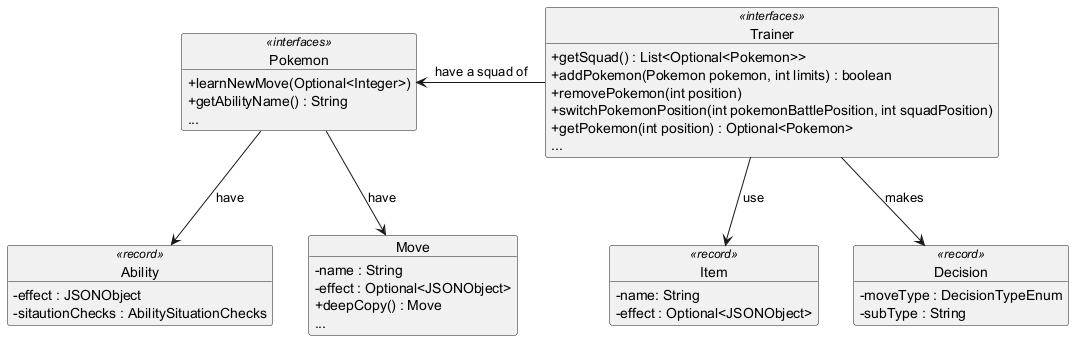
\includegraphics[width=\textwidth]{immagini/modello.png}
\caption{Schema UML dell'analisi del problema, con rappresentate le entità principali ed i rapporti fra loro}
\end{figure}

\chapter{Design}

\section{Architettura}

L'architettura del gioco PokéRogue adotta il patternMVC (Model-View-Controller), che consente una chiara separazione delle responsabilità e una maggiore flessibilità nello sviluppo. Grazie a questa struttura, è possibile sostituire intere componenti della {View senza influire sul Controller  o sul Model. Questa suddivisione favorisce inoltre lo sviluppo modulare, in cui ogni parte può essere implementata e testata isolatamente. La comunicazione tra i componenti MVC avviene tramite metodi definiti nelle interfacce, garantendo una struttura coerente e facilmente estendibile.\\
L’architettura del progetto si basa su cinque elementi principali:
\begin{itemize}
    \item \textbf{Scene}
    \item \textbf{GameEngine}
    \item \textbf{GraphicEngine}
    \item \textbf{KeyListener}
\end{itemize}
Il \textbf{GameEngine} svolge un ruolo centrale, coordinando la comunicazione tra le Scene, il KeyListener e il GraphicEngine. Il gioco si sviluppa attorno a un ciclo semplice ma efficace: il KeyListener intercetta gli input da tastiera e li inoltra al GameEngin}, che contiene un riferimento alla Scene attiva, alla quale delega l’elaborazione dell’input.\\
La Scene gestisce l’input aggiornando lo stato interno e modificando di conseguenza gli elementi visivi attraverso la SceneView. Inoltre, ogni Scene interagisce con i componenti del Model per eseguire operazioni come:
\begin{itemize}
    \item Caricare i Pokémon da un salvataggio
    \item Salvare una partita
    \item Caricare le caratteristiche degli elementi grafici
    \item Eseguire altre funzionalità di gioco
\end{itemize}

Infine, il \textbf{GameEngine} agisce come intermediario tra la \textbf{Scene} attiva e il \textbf{GraphicEngine}: per ogni ciclo di esecuzione, recupera dalla \textbf{Scene} l'elenco aggiornato degli elementi grafici da visualizzare e li trasmette al \textbf{GraphicEngine}, che ne gestisce il posizionamento e la renderizzazione a schermo. Questo meccanismo viene ripetuto a ogni input dell'utente, assicurando che ogni tasto premuto sulla tastiera produca un aggiornamento immediato e visibile dell'interfaccia di gioco.


\begin{figure}[h]
\centering{}
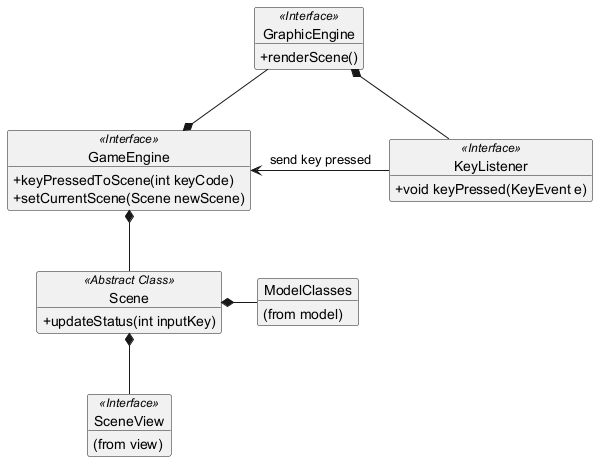
\includegraphics[width=9cm]{immagini/architetturaMVC.png}
\caption{Diagramma UML che rappresenta l'architettura del progetto, evidenziando l'adozione del pattern architetturale MVC.}

\end{figure}






\section{Design dettagliato}


\subsection{Egor Tverdohleb}
\subsection*{Generazione dei Pokemon}
\begin{figure}[H]
\centering{}
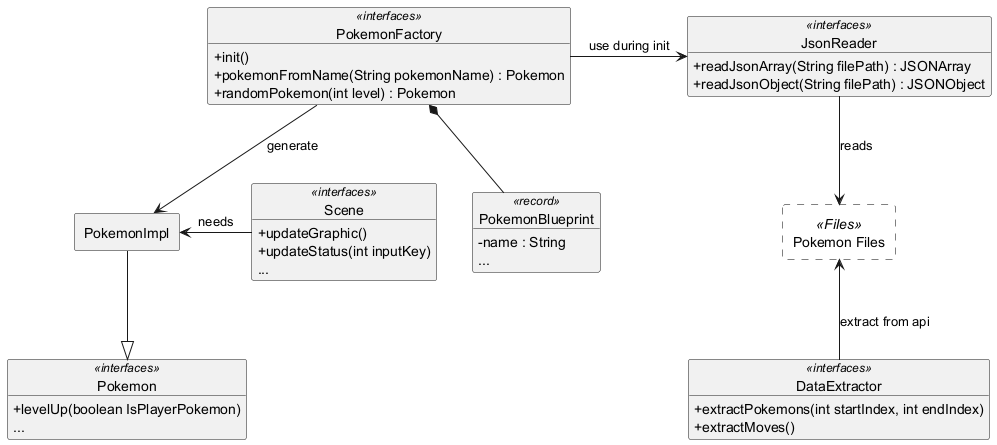
\includegraphics[width=\textwidth]{immagini/pokemonFactory.png}
\caption{Rappresentazione UML della pokemon Factory}
\label{immagini/pokemonFactory}
\end{figure}
\paragraph{Problema}
È necessario implementare un sistema di generazione dei Pokémon tenendo conto che condividono un insieme di valori fissi determinati dalla loro specie, ma presentano anche alcune caratteristiche che devono essere generate casualmente al momento della creazione.

\paragraph{Soluzione} Per gestire in modo efficiente la creazione dei Pokémon, è stato adottato il \textit{pattern Factory}. I dati statici relativi a ciascuna specie di Pokémon sono stati estratti e salvati in appositi file JSON. In particolare si è costruito un DataExtractor per utilizzare la REST API pokeApi {\footnote{\url{https://pokeapi.co//}}. Per evitare accessi ripetuti al file system e ridurre i tempi di caricamento percepiti dall’utente, tali dati vengono caricati una sola volta durante l’inizializzazione del gioco e mantenuti in memoria. La \texttt{PokemonFactory} si occupa della lettura dei file JSON e della memorizzazione dei relativi oggetti \texttt{PokemonBlueprint} in una struttura indicizzata. I metodi esposti dalla factory consentono di creare nuovi Pokémon clonando le informazioni fisse dal blueprint corrispondente e completandole con valori generati casualmente (es. statistiche variabili, abilità, ecc.). In questo modo, il sistema garantisce efficienza nella generazione dei Pokémon e coerenza tra gli esemplari della stessa specie.
\subsection*{Gestione degli effetti}
\begin{figure}[H]
\centering{}
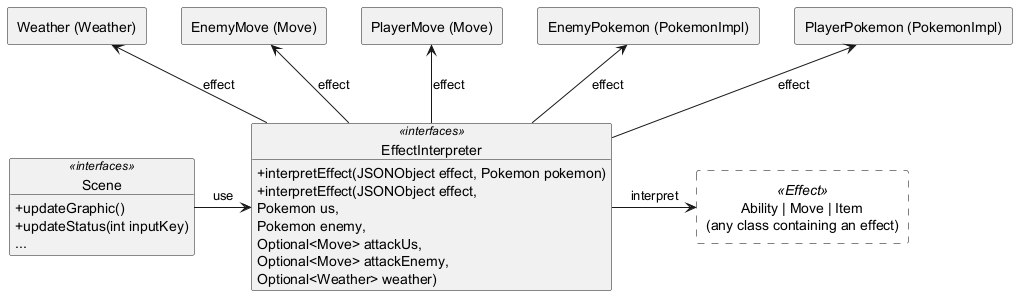
\includegraphics[width=\textwidth]{immagini/effectInterpreter.png}
\caption{Rappresentazione UML della gestione degli effetti}
\label{immagini/effectInterpreter}
\end{figure}
\paragraph{Problema}
Si desidera gestire Abilità, Mosse e Oggetti considerando che ognuno ha un effetto specifico. Ogni effetto deve essere applicato in modo contestuale alla battaglia in corso.

\paragraph{Soluzione}
Come descritto nella fase di modellazione, il concetto di effetto è stato unificato e strutturato secondo la seguente rappresentazione all'interno dei rispetti file JSON:

\begin{itemize}
    \item \textbf{checks}: lista di liste di stringhe.

    Ogni elemento della lista rappresenta un singolo \textit{check}, composto da tre stringhe nel formato:
    \begin{center}
        \texttt{Valore1 \ Segno \ Valore2}
    \end{center}

    \begin{itemize}
        \item \texttt{Valore1} e \texttt{Valore2} rappresentano rispettivamente un parametro (o campo) e un valore atteso, e possono fare riferimento a costanti (es. \texttt{enum}) o a proprietà dell'entità in gioco.
        \item \texttt{Segno} indica un operatore logico tra i seguenti: \texttt{==, \(\geq\), \(>\), \(\leq\), \(<\), !=}.
    \end{itemize}

    Un insieme di \texttt{check} è considerato valido se tutte le condizioni in esso presenti risultano vere contemporaneamente.

    \item \textbf{activations}: lista di liste di stringhe.

    Ogni elemento rappresenta un’\textit{activation}, ovvero un'azione che modifica uno stato del sistema. È composta da due stringhe:
    \begin{itemize}
        \item \texttt{Valore1}: il nome del parametro o campo da modificare.
        \item \texttt{Valore2}: il nuovo valore da assegnare a \texttt{Valore1}.
    \end{itemize}
\end{itemize}In questo modo è stato possibile definire un EffectInterpreter seguendo il \textit{pattern Interpreter} lasciando grande elasticità al sistema per l'aggiunta di nuove abilita, mosse o ogetti
\subsection*{Generazione delle Abilita e Mosse}
\begin{figure}[H]
\centering{}
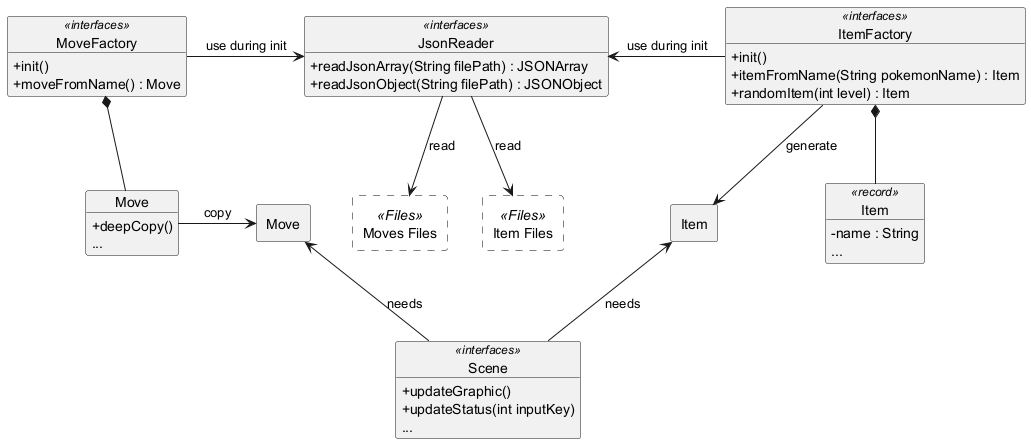
\includegraphics[width=\textwidth]{immagini/MoveAbilityFactory.png}
\caption{Rappresentazione UML delle Move e Ability Factory}
\label{immagini/MoveAbilityFactory}
\end{figure}
\paragraph{Problema} Si desidera generare Abilità e Mosse, tenendo considerazione dell'overhead causato dalla lettura in memoria
\paragraph{Soluzione} Il problema risulta sostanzialmente analogo a quello della generazione dei Pokémon, e viene affrontato con una soluzione simile, con alcuni accorgimenti specifici. Le Abilità, non necessitando di modificare i propri campi, sono state modellate come oggetti immutabili. Seguendo il \textit{pattern Factory}, è stata realizzata una classe factory incaricata di effettuare un’unica lettura dei dati da memoria all’avvio, per poi restituire le istanze appropriate su richiesta.
Le Mosse, al contrario, richiedono uno stato interno modificabile e sono quindi state modellate come oggetti mutabili. Per mantenere l’efficienza del singolo accesso in memoria, alla factory è stato affiancato l’utilizzo del \textit{pattern Prototype}, permettendo di restituire copie delle mosse originali ogni volta che vengono richieste.

\subsection{Maretti Pietro}
\subsection*{Creazione di un'intelligenza artificiale per i nemici}


\begin{figure}[H]
\centering{}
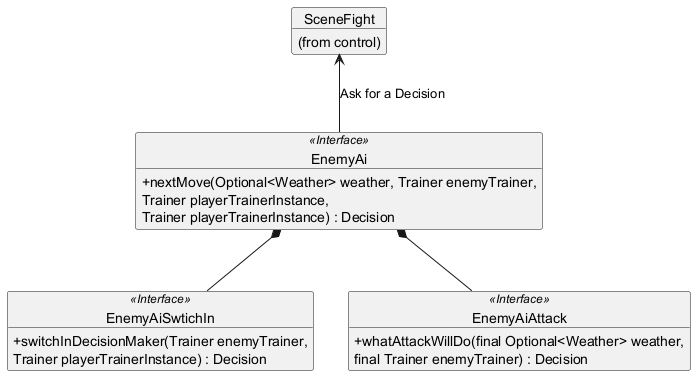
\includegraphics[width=\textwidth]{immagini/AiUml.png}
\caption{Schema UML che raffigura come la SceneFight utilizza l'Ai e di come essa divide il suo compito }
\label{immagini/AiUml.png}
\end{figure}
\paragraph{Problema} 
Nel contesto del gioco, si desidera implementare un sistema di intelligenza artificiale in grado di prendere decisioni per un nemico durante i combattimenti. Tale sistema deve adattarsi a diversi livelli di difficoltà, influenzando la complessità e l'efficacia delle scelte effettuate dall'IA.\\

\paragraph{Soluzione}Per gestire queste scelte è stata definita l'interfaccia \texttt{EnemyAI}, che espone il metodo \texttt{nextMove}. Questo metodo restituisce un oggetto di tipo \texttt{Decision} e accetta i seguenti parametri:

\begin{itemize}
    \item un \texttt{Optional<Weather>}, che rappresenta le condizioni atmosferiche attuali
    \item il \texttt{Trainer} del giocatore
    \item il \texttt{Trainer} nemico (controllato dall'IA)
\end{itemize}

La classe \texttt{EnemyAiImpl}, che implementa l'interfaccia, riceve in fase di costruzione il livello di difficoltà. Tale valore viene utilizzato per impostare delle flag interne che influenzano il processo decisionale, rendendolo più o meno sofisticato.\\Quando viene richiesta la prossima mossa, la classe \texttt{EnemyAimpl} utilizza due classi di supporto create segundo il \textit{pattern} \textit{Separation of concerns}: \texttt{EnemyAiSwitchIn} e \texttt{EnemyAiAttack}.\\
Viene invocato il metodo \texttt{switchInDecisionMaker()} della classe \texttt{EnemyAiSwitchIn}, che valuta le condizioni della battaglia e le flag impostate per decidere se effettuare uno switch e, in tal caso, quale Pokémon mandare in campo. Se questo metodo non restituisce una decisione valida, si procede con la chiamata al metodo \texttt{whatAttackWillDo()} della classe \texttt{EnemyAiAttack}, che valuta se attaccare e quale mossa utilizzare.\\
Il primo tra questi due metodi che restituisce una decisione valida fornisce il risultato finale, che viene restituito da \texttt{EnemyAiImpl} come mossa scelta dall'intelligenza artificiale.\\
Nel caso in cui non venga scelta né un'azione di switch né un attacco ad esempio per via dell'impossibilità di agire o dell'inutilità di qualsiasi scelta disponibile l'oggetto \texttt{Decision} risulterà vuoto. In tal caso, il nemico non eseguirà alcuna azione durante il turno corrente.\\
\subsection*{Creazione di un sistema grafico flessibili e che si adatti allo schermo}


\begin{figure}[H]
\centering{}
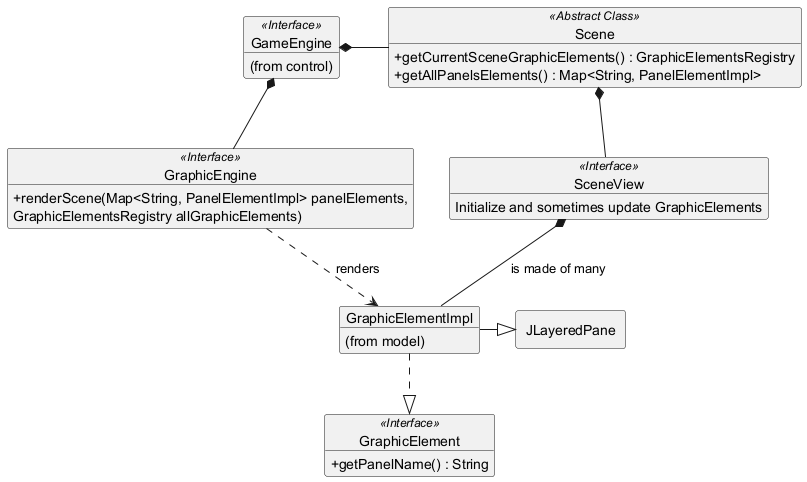
\includegraphics[width=\textwidth]{immagini/GraphicsUml.png}
\caption{Schema UML che mostra il legame fra i GraphicElements le Scene, il GraphicEngine e il GameEngine }
\label{immagini/GraphicsUml.png}
\end{figure}

\paragraph{Problema} 
Il gioco deve avere una struttura grafica altamente flessibile, in grado di gestire componenti eterogenei come box, sprite, sfondi e testi. L'obiettivo è evitare vincoli rigidi imposti dai layout tradizionali, pur garantendo un comportamento adattivo: l'interfaccia deve essere in grado di ridimensionarsi automaticamente al variare delle dimensioni della schermata.

\paragraph{Soluzione}
La grafica del gioco si basa su due componenti principali: i \texttt{GraphicElement} e il \texttt{GraphicEngine}. I primi rappresentano gli elementi visivi che compongono una scena, mentre il secondo è responsabile della loro visualizzazione a schermo.\\La classe \texttt{GraphicElementImpl} implementa l'interfaccia \texttt{GraphicElement} ed estende \texttt{JLayeredPane}. Ogni \texttt{GraphicElement} è quindi un pannello personalizzato, all'interno del quale vengono disegnati i contenuti grafici tramite il metodo \texttt{paintComponent()}, che consente di renderizzare box, testi, immagini e altri elementi visivi.\\
Sono stati definiti sei tipi principali di \texttt{GraphicElement}, ciascuno dei quali estende \texttt{GraphicElementImpl} e ridefinisce il metodo \texttt{paintComponent()} in base alle proprie esigenze. Gli elementi fondamentali sono:
\begin{itemize}
    \item \texttt{BoxElement}: un contenitore grafico generico;
    \item \texttt{SpriteElement}: utilizzato per visualizzare immagini;
    \item \texttt{TextElement}: per la gestione e visualizzazione del testo;
    \item \texttt{ButtonElement}: un wrapper di \texttt{BoxElement} che aggiunge la funzione \texttt{setSelected()}, utile per evidenziare il bordo del pulsante quando selezionato;
    \item \texttt{BackgroundElement}: un wrapper di \texttt{SpriteElement}, utilizzato per visualizzare immagini di sfondo a schermo intero.
\end{itemize}
Ogni \texttt{GraphicElement} può essere istanziato specificando manualmente parametri come posizione, dimensioni e stile, oppure tramite un costruttore che accetta un oggetto \texttt{JSONObject}. Quest’ultima modalità consente di caricare la configurazione degli elementi da file JSON, rendendo flessibile la definizione delle scene grafiche.\\
Le coordinate e le dimensioni sono espresse come percentuali rispetto alla risoluzione dello schermo, garantendo un ridimensionamento automatico e proporzionale degli elementi al variare della finestra di gioco.\\
Per gestire la profondità e la disposizione degli elementi, è stata introdotta l'interfaccia \texttt{PanelElement}, che rappresenta un contenitore dotato di \texttt{Layout}, configurabile tramite il costruttore. Questo consente di suddividere ogni scena in più layer e di controllare accuratamente la sovrapposizione degli elementi grafici.\\
Tutti i \texttt{GraphicElement} vengono assegnati a un \texttt{PanelElement}. Durante la fase di rendering, il \texttt{GraphicEngine} utilizza il metodo \texttt{getPanelName()} di ciascun elemento per determinarne il pannello di appartenenza e visualizzarlo correttamente nella scena.\\
L’intera architettura grafica si basa sul \textit{Composite Pattern}. In questo contesto, ogni scena (\texttt{View}) è modellata come una gerarchia di elementi: i \texttt{GraphicElement} fungono da componenti foglia (\textit{leaf}), ovvero elementi grafici atomici e non suddivisibili, mentre i \texttt{PanelElement} rappresentano i compositi (\textit{composite}), in quanto possono contenere altri \texttt{GraphicElement}, compresi altri \texttt{PanelElement}. Questo approccio consente di strutturare l’interfaccia in maniera modulare, flessibile e scalabile.\\



\subsection*{Aggiungere e far selezionare i pokèmon al giocatore prima di iniziare la run}


\begin{figure}[H]
\centering{}
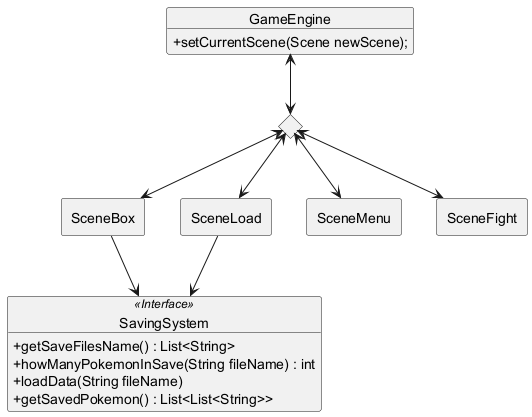
\includegraphics[width=\textwidth]{immagini/MenuLoadBoxuml.png}
\caption{Schema UML che raffigura le connessioni fra le Scene: Menu, Load, Box e Fight rispetto al GameEngine. }
\label{immagini/MenuLoadBoxuml.png}
\end{figure}

\paragraph{Problema} 
All'avvio di una run, il giocatore deve poter selezionare i Pokémon con cui iniziare. Questa selezione deve avvenire caricando un set di Pokémon da un salvataggio precedente, oppure iniziando da una nuova box contenente i tre Pokémon iniziali predefiniti.
\paragraph{Soluzione}
Per far selezionare al giocatore la squadra iniziale in una delle due modalità all'avvio del gioco, viene mostrato all'avvio del gioco o alla fine di ogni run la \texttt{SceneMenu}, che permette di iniziare una nuova run scegliendo tra due opzioni: caricare un salvataggio esistente oppure partire con la box iniziale contenente i tre Pokémon starter.\\
Nel caso in cui il giocatore scelga di caricare un salvataggio, la \texttt{SceneMenu} richiama il \texttt{GameEngine}, che provvede a passare il controllo alla \texttt{SceneLoad}. Questa scena si occupa di caricare tutti i salvataggi disponibili dalla cartella dedicata, utilizzando il \texttt{SavingSystem}. Una volta visualizzati, la \texttt{SceneLoad} consente di scorrere e selezionare uno dei salvataggi. Il file selezionato viene quindi passato come parametro alla \texttt{SceneBox} tramite il \texttt{GameEngine}.\\
Nel caso si opti invece per una nuova partita, viene comunque utilizzata la stessa \texttt{SceneBox}, ma inizializzata con una stringa vuota nel costruttore. Questo indica alla \texttt{SceneBox} che non deve essere effettuato alcun caricamento da file, ma devono essere invece mostrati i Pokémon starter di default.\\
Indipendentemente dal percorso scelto, la \texttt{SceneBox} ha il compito di mostrare al giocatore la lista dei Pokémon disponibili (da salvataggio o predefiniti) e permettere la selezione di un massimo di tre Pokémon con cui iniziare la run. Ogni volta che un Pokémon viene selezionato, esso viene aggiunto alla squadra del \texttt{Trainer} del giocatore; in caso di deselezione, il Pokémon viene rimosso dalla squadra.\\
Una volta selezionato almeno un Pokémon, il giocatore può avviare ufficialmente la run premendo il pulsante di \texttt{Start}, il quale richiama l'inizializzazione della scena di combattimento, la \texttt{SceneFight}.

\subsection{Miraglia Tommaso Cosimo}
\subsection*{Gestione del turno di battaglia}
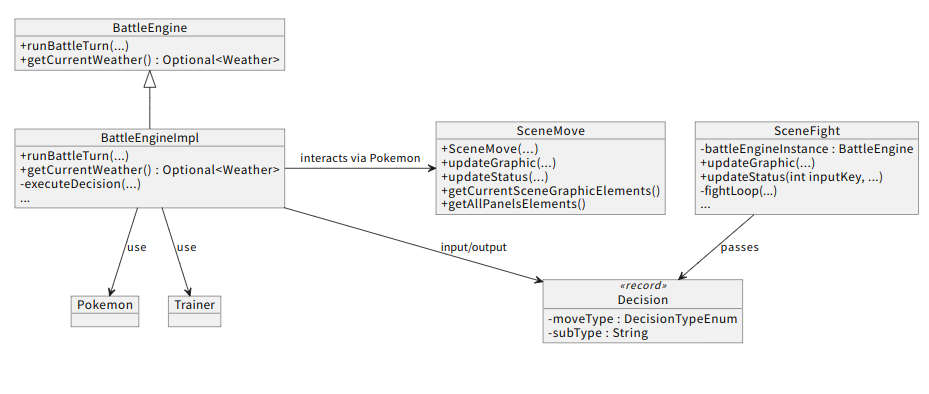
\includegraphics[width=\textwidth]{immagini/battleEngineUML.png}
\paragraph{Problema}
Nel contesto del gioco, è necessario un sistema in grado di orchestrare le dinamiche di combattimento tra il giocatore e un nemico, tenendo conto di numerosi fattori come le mosse selezionate, gli effetti delle abilità, le condizioni meteorologiche, i cambi di Pokémon, e l’interazione con un’eventuale intelligenza artificiale. Questo sistema deve anche integrare meccanismi per la cattura dei Pokémon, l’assegnazione delle ricompense e la gestione della progressione del giocatore.

\paragraph{Soluzione}
Per affrontare questo problema è stata sviluppata la classe\linebreak 
\texttt{BattleEngineImpl}, un’implementazione dell’interfaccia \texttt{BattleEngine}. Questa classe si occupa della gestione completa del turno di battaglia e coordina le azioni del giocatore e del nemico, comprese quelle decise dall'intelligenza artificiale.\\
Il metodo principale, \texttt{runBattleTurn}, riceve le decisioni del giocatore e del nemico (sotto forma di oggetti \texttt{Decision}) e, a partire dalla priorità delle mosse e dalla velocità dei Pokémon, stabilisce l’ordine di esecuzione. Durante l’esecuzione, vengono valutati e applicati eventuali effetti di abilità (\texttt{handleAbilityEffects}), condizioni di stato (\texttt{applyStatusForAllPokemon}) e danni derivanti da attacchi (\texttt{handleAttack}).\
Se una delle due decisioni prevede l’uso di una Pokéball, il metodo \texttt{handlePokeball} viene invocato per determinare l’esito della cattura, aggiornare il salvataggio e, se necessario, modificare lo stato della partita.\
In caso di sconfitta del Pokémon nemico o di cambio forzato, viene effettuato un controllo tramite il metodo \verb|newEnemyCheck|, che gestisce l’eventuale ingresso di un nuovo avversario oppure il passaggio a una fase successiva della partita, come lo shop o il salvataggio finale.\\
Il design della classe adotta un approccio modulare, delegando le responsabilità specifiche (calcolo del danno, applicazione effetti, cambio Pokémon) a metodi separati, seguendo il principio della \textit{Separation of Concerns}. L’integrazione con altre componenti del gioco (es. \texttt{GameEngine}, \texttt{SavingSystem}) consente di mantenere aggiornata la progressione del giocatore e l’evoluzione della battaglia.

\subsection*{Implementazione della scena di combattimento}
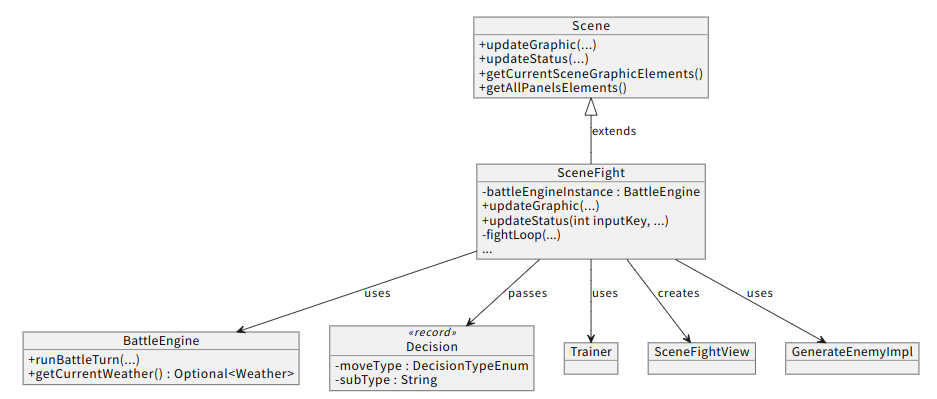
\includegraphics[width=\textwidth]{immagini/sceneFightUML.png}

\paragraph{Problema}
Gestire la scena di combattimento nel gioco, coordinando input utente, aggiornamenti grafici e logica di battaglia, inclusa la generazione del nemico.

\paragraph{Soluzione}
La classe \texttt{SceneFight} estende \texttt{Scene} e rappresenta il controller principale della scena di combattimento, orchestrando l’interazione tra l’input utente, la logica di battaglia e la visualizzazione grafica. Al suo interno, la classe gestisce l’inizializzazione e il mantenimento dello stato del trainer nemico tramite \texttt{TrainerImpl}, e crea un’istanza di intelligenza artificiale avversaria mediante \texttt{EnemyAiImpl}, configurata in base al livello di difficoltà della battaglia.\\
La gestione degli input da tastiera avviene tramite il metodo \texttt{updateStatus}, il quale interpreta i comandi dell’utente aggiornando la selezione corrente o attivando l’esecuzione delle azioni corrispondenti, come attacchi, uso di oggetti o cambio di Pokémon. In particolare, l’input è mappato su codici interni che rappresentano le varie azioni disponibili, consentendo una navigazione fluida e coerente tra i diversi elementi dell’interfaccia.\\
Quando l’utente conferma un’azione, la classe richiama \texttt{fightLoop}, che invoca il metodo \texttt{nextMove} dell’istanza di \texttt{EnemyAi} per ottenere la decisione strategica del nemico. Successivamente, tramite \texttt{BattleEngine.runBattleTurn}, vengono elaborate simultaneamente entrambe le decisioni (giocatore e IA), aggiornando lo stato della battaglia.\\
L’aggiornamento degli elementi grafici è affidato a \texttt{SceneFightView}, che riflette in tempo reale lo stato della scena, assicurando una sincronizzazione visiva con le scelte e gli eventi di gioco. La struttura complessiva garantisce così una chiara separazione tra gestione degli input, logica di combattimento e rendering grafico, permettendo un’architettura modulare, scalabile e facilmente manutenibile.

\subsection*{Generazione Dinamica degli Avversari}
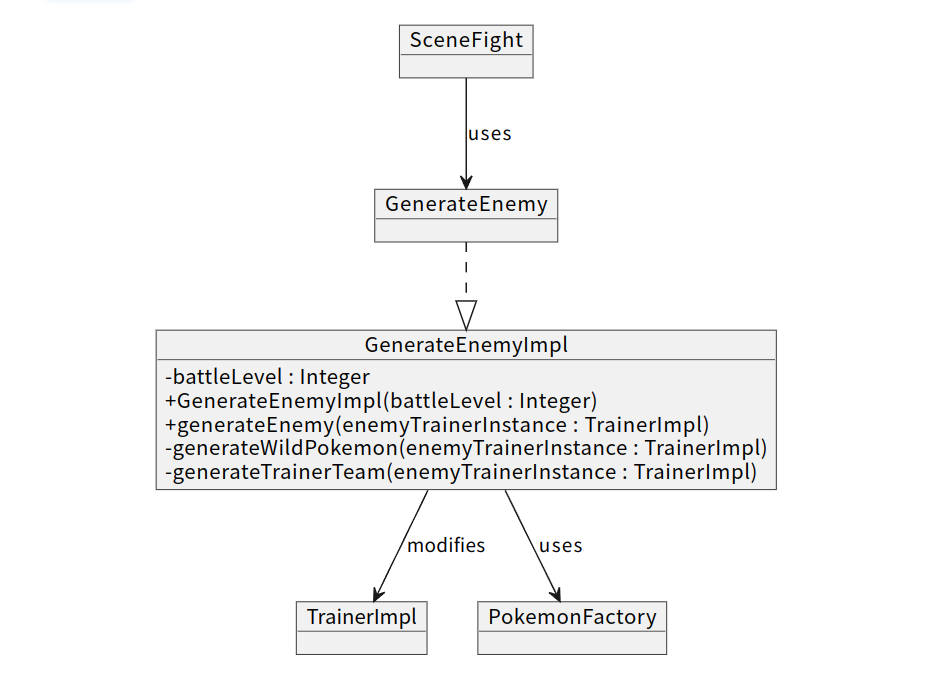
\includegraphics[width=\textwidth]{immagini/generateEnemyUML.png}
\paragraph{Problema}
Nel contesto del sistema di combattimento, è necessario generare nemici che siano coerenti con il livello di difficoltà e il contesto della battaglia, differenziando tra Pokémon selvatici e allenatori avversari, e gestendo le relative implicazioni di gameplay come la possibilità di cattura.

\paragraph{Soluzione}
La classe \texttt{GenerateEnemyImpl} si occupa di creare nemici adeguati al livello di battaglia. Il sistema prevede due tipologie di avversari: Pokémon selvatici e allenatori nemici con una squadra completa di Pokémon. Nel dettaglio, quando il livello della battaglia è un multiplo di cinque, viene generato un allenatore nemico dotato di una squadra composta da più Pokémon, il cui numero cresce in base al livello, fino a un massimo stabilito. In caso contrario, si genera un singolo Pokémon selvatico, contraddistinto da uno stato che ne permette la cattura durante il combattimento.
I livelli dei Pokémon, sia selvatici che della squadra degli allenatori, sono calcolati in base al livello della battaglia, con una componente casuale che introduce variazioni per aumentare la varietà degli incontri. La generazione degli specifici Pokémon è delegata a una factory dedicata che crea istanze coerenti con il livello stabilito.
Questa distinzione tra nemici offre una differenziazione importante nel gameplay: i Pokémon selvatici rappresentano incontri occasionali che il giocatore può catturare e aggiungere alla propria squadra, mentre i Pokémon degli allenatori sono avversari fissi che non possono essere catturati, ma devono essere sconfitti per progredire. In questo modo, la generazione dinamica degli avversari contribuisce a creare una progressione di difficoltà bilanciata e un’esperienza di gioco varia e coinvolgente.

\subsection{Casadio Alex}
\subsection*{Gestione della scena di salvataggio}

\begin{figure}[H]
\centering{}
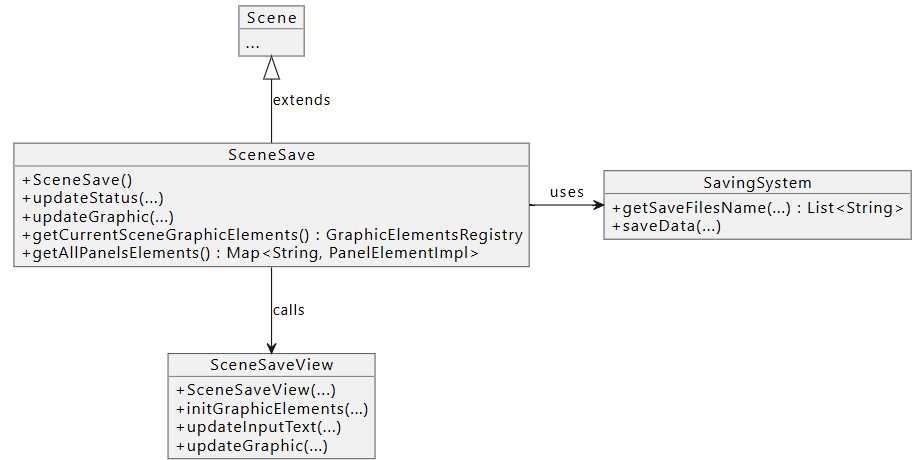
\includegraphics[width=\textwidth]{immagini/sceneSaveUml.png}
\caption{Schema UML che raffigura la scena di salvataggio. }
\label{immagini/MenuLoadBoxuml.png}
\end{figure}

\paragraph{Problema}
Era necessario implementare una schermata di salvataggio che consentisse all’utente di inserire un nome, verificare eventuali conflitti con salvataggi esistenti e scegliere se continuare o uscire salvando.

\paragraph{Soluzione}
La classe \texttt{SceneSave} estende \texttt{Scene} ed è responsabile della gestione logica e grafica della schermata di salvataggio. Vengono inizializzati gli elementi grafici tramite file JSON, seguendo lo stesso approccio delle altre scene. I pulsanti sono mappati attraverso una struttura dati che associa i nomi degli elementi a interi, rendendo più semplice gestirne lo stato.\

La scena gestisce due pulsanti principali: "EXIT\_AND\_SAVE" e \linebreak "EXIT\_WITHOUT\_SAVING". L'input dell'utente viene elaborato tramite il metodo \texttt{updateStatus()}, che si occupa della navigazione tra i pulsanti e dell’attivazione delle azioni. In particolare:
\begin{itemize}
\item Premendo \texttt{Enter} su "EXIT\_WITHOUT\_SAVING", il gioco ritorna alla scena principale.
\item Premendo \texttt{Enter} su "EXIT\_AND\_SAVE", si attiva una procedura di salvataggio.
\end{itemize}

Il salvataggio viene effettuato solo se il nome inserito non è già presente tra i file nella directory \texttt{resources/saves}. In caso contrario, l’utente riceve un messaggio che lo informa del conflitto.\\
L’inserimento del nome avviene tramite il metodo \texttt{handleTextInput()}, che gestisce lettere, numeri, spazi e il tasto \texttt{Backspace}. Il nome inserito è limitato a una lunghezza massima, per evitare problemi di visualizzazione o salvataggio.\\
La classe interagisce con il sistema di salvataggio e con il motore grafico, aggiornando dinamicamente i contenuti a schermo tramite la classe \texttt{SceneSaveView}. Tutti gli elementi grafici vengono inseriti in un \linebreak \texttt{GraphicElementsRegistry} temporaneo e poi utilizzati per il rendering.\\
Questa scena rappresenta un buon esempio di coordinazione tra logica di gioco, gestione dell’input utente e flessibilità grafica. È stata progettata per essere facilmente estendibile e integrabile con il resto dell’architettura.

\subsection*{Gestione dell'acquisto ed utilizzo di items}

\begin{figure}[H]
\centering{}
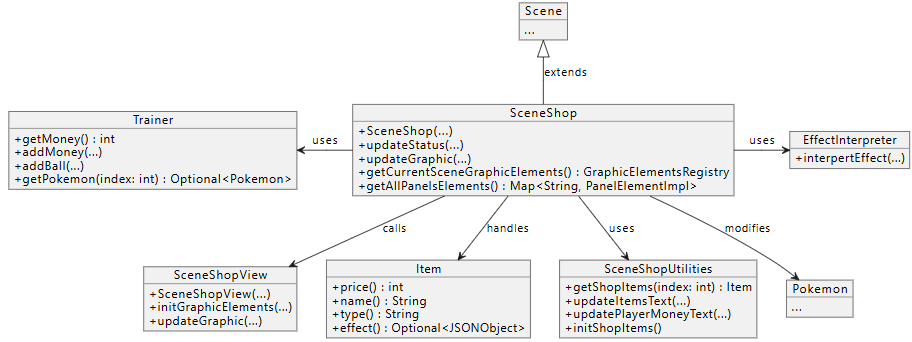
\includegraphics[width=\textwidth]{immagini/sceneShopUml.png}
\caption{Schema UML che raffigura la scena dello shop. }
\label{immagini/MenuLoadBoxuml.png}
\end{figure}

\paragraph{Problema}
Era necessario creare un’interfaccia interattiva che permettesse al giocatore di acquistare, usare oggetti e gestire il proprio team Pokémon durante la fase di “Shop”, garantendo navigazione fluida e feedback coerente.

\paragraph{Soluzione}  
Per affrontare la complessità derivante dalla gestione di molteplici elementi interattivi con comportamenti diversi, la progettazione di \texttt{SceneShop} si è basata su alcuni principi fondamentali: separazione della logica, astrazione delle interazioni utente e modularità della visualizzazione.\\
Il primo passo è stato quello di rappresentare ogni elemento grafico (pulsanti per oggetti, comandi, squadra) tramite un nome simbolico associato a un intero. Questa associazione è memorizzata all’interno di una mappa (\texttt{graphicElementNameToInt}), che permette una navigazione efficiente e flessibile, evitando la necessità di hardcodare indici numerici. In questo modo, il codice resta facilmente adattabile a eventuali modifiche nella disposizione o nel numero di pulsanti.\\
Un’altra scelta fondamentale è stata quella di distinguere chiaramente tra lo stato corrente del cursore (\texttt{currentSelectedButton}) e quello verso cui si sta navigando (\texttt{newSelectedButton}). Questa distinzione ha permesso di implementare meccaniche di evidenziazione visiva e di aggiornamento progressivo dello stato, consentendo ad esempio animazioni o transizioni fluide nel rendering.\\
La logica di navigazione (gestita in \texttt{updateStatus()}) è strutturata tramite controlli condizionali che verificano in quale “zona” del negozio si trovi l’utente: oggetti gratuiti, oggetti acquistabili, pulsanti speciali, o selezione dei Pokémon. Per ciascuna zona vengono applicate regole di spostamento coerenti: ad esempio, nel caso dei Pokémon, la navigazione avviene in senso orizzontale, mentre per i pulsanti oggetto è verticale.\\
L'acquisto e l'uso degli oggetti sono stati separati in due momenti logici. Alla pressione di \texttt{Enter} su un oggetto acquistabile, viene verificata la disponibilità di denaro e, in caso positivo, l'oggetto viene segnato come "in attesa di utilizzo" (\texttt{selectedItemForUse = true}) e si apre la schermata di selezione del Pokémon. Una volta che il giocatore seleziona un Pokémon, viene invocato \texttt{applyItemToPokemon()}, che interpreta l’effetto dell’oggetto tramite l’\texttt{EffectInterpreter} e lo applica al soggetto scelto.\\
Nel caso in cui il giocatore decida di tornare indietro senza applicare l’oggetto, viene attivata una procedura di \texttt{compensazione} (metodo \texttt{compensation()}), che rimborsa il denaro speso. Questo garantisce che nessuna risorsa venga persa a causa di input accidentali o ripensamenti, migliorando l’esperienza utente e la robustezza del sistema.\\
Il \texttt{reroll} degli oggetti è stato trattato come operazione distinta, con un costo fisso. La sua logica è incapsulata in un metodo dedicato (\texttt{rerollShopItems()}), che aggiorna le descrizioni degli oggetti a schermo e scala la quantità di denaro del giocatore. Questo approccio favorisce la riusabilità del codice in altri contesti futuri (ad esempio, mercati diversi o oggetti temporanei).\\
Per la parte grafica, la classe delega il disegno degli elementi a \texttt{SceneShopView}, seguendo il principio di separazione tra logica e presentazione. Ogni aggiornamento visivo è guidato da un registro di elementi (\texttt{GraphicElementsRegistry}) che viene aggiornato dinamicamente in risposta alle azioni dell’utente.\\
Infine, l’intero design della scena è stato pensato per essere facilmente estendibile: l’aggiunta di nuovi oggetti, comandi, o tipologie di interazioni può avvenire con interventi minimi sulla logica principale, mantenendo la compatibilità con il motore grafico e con le altre componenti del gioco.

\subsection*{Creazione degli items}

\begin{figure}[H]
\centering{}
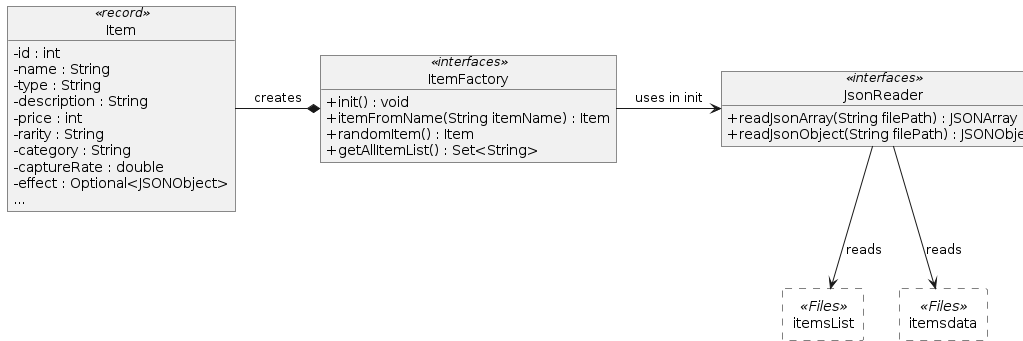
\includegraphics[width=\textwidth]{immagini/itemFactoryUml.png}
\caption{Schema UML che raffigura l'itemFactory. }
\label{immagini/MenuLoadBoxuml.png}
\end{figure}

\paragraph{Problema}
Nel contesto del gioco, è necessario gestire una grande quantità di oggetti con caratteristiche diverse, definite esternamente in file JSON. È importante garantire un accesso rapido e sicuro a queste informazioni, evitando letture ridondanti da disco e potenziali incoerenze. Inoltre, si desidera poter accedere agli oggetti sia per nome che in maniera casuale, ad esempio durante la generazione del negozio o il drop di premi.

\paragraph{Soluzione}
La soluzione adottata consiste nell’utilizzare un approccio centralizzato tramite la classe \texttt{ItemFactory}, che funge da punto unico di accesso e gestione per tutti gli oggetti. La fase di inizializzazione (\texttt{init()}) legge in anticipo tutti i file JSON e popola una mappa contenente oggetti immutabili. Questa scelta consente:
\begin{itemize}
\item di evitare letture ripetute da disco durante il gioco, migliorando l’efficienza;
\item di garantire che ogni oggetto esista in una sola versione coerente (immutabilità del record \texttt{Item});
\item di semplificare l’accesso e la gestione degli oggetti tramite nomi simbolici.
\end{itemize}
L’utilizzo di \texttt{Optional<JSONObject>} per rappresentare l’effetto consente di gestire in modo elegante la presenza o assenza di un comportamento speciale associato all’oggetto. Inoltre, la funzione \texttt{randomItem()} sfrutta un \texttt{Set} e uno \texttt{Stream} per selezionare un oggetto casuale, mantenendo l’implementazione semplice ma efficace.\\
L’intero design è facilmente estendibile: per aggiungere un nuovo oggetto, è sufficiente aggiornare il file \texttt{itemsList.json} e fornire il relativo file \texttt{.json} con le specifiche. Questo approccio favorisce la modularità, la scalabilità e la manutenzione del progetto.










\chapter{Sviluppo}

\section{Testing automatizzato}
In questo progetto abbiamo deciso di testare le principali classi del Model utilizzando la suite \textit{JUnit}.

Riportiamo brevemente i componenti che abbiamo sottoposto a test automatizzato:
\begin{itemize}
    \item \texttt{MoveFactory}: viene verificata la corretta creazione delle mosse, la loro potenza, precisione, tipo e PP.
    \item \texttt{AbilityFactory}: viene testata la corretta istanziazione delle abilità, verificando che le condizioni di attivazione siano correttamente interpretate.
    \item \texttt{Move copy}: viene verificato che oggetti \texttt{Move} uguali siano distinti in memoria e che modifiche su uno non influenzino l'altro.
    \item \texttt{EffectInterpreter su mosse}: viene testata l'interpretazione degli effetti delle mosse a partire da un file JSON.
    \item \texttt{EffectInterpreter su abilità}: viene testata l'applicazione corretta degli effetti delle abilità da file JSON.
    \item \texttt{PokeEffectivenessCalc}: viene verificata la correttezza del calcolo dell’efficacia degli attacchi tra diversi tipi di Pokémon.
    \item \texttt{EffectInterpreter su oggetti}: viene verificata l’applicazione corretta degli effetti degli oggetti su un Pokémon e sul trainer.
    \item \texttt{PPItemsTest}: viene testato il corretto funzionamento dell’oggetto \texttt{Elixir}, assicurandosi che ripristini tutti i PP delle mosse.
    \item \texttt{AI}: viene testata la logica decisionale dell'intelligenza artificiale, verificando che venga scelta l’azione più coerente in funzione del contesto.
    \item \texttt{BattleRewards}: viene verificato che, al termine della battaglia, l’esperienza venga correttamente assegnata al Pokémon del vincitore.
    \item \texttt{GenerateEnemyInstance}: viene verificata la corretta generazione di un avversario con un numero coerente di Pokémon nella squadra.
    \item \texttt{BattleEngine con decisione NOTHING}: viene testato il comportamento del motore di battaglia quando il giocatore non compie alcuna azione.
    \item \texttt{BattleEngine con Pokéball}: viene testata la cattura di un Pokémon avversario utilizzando una Masterball, controllando che entri nella squadra del giocatore.
    \item \texttt{BattleEngine con cambio Pokémon}: viene verificata la corretta gestione del cambio Pokémon durante una battaglia.
    \item \texttt{GameEngine - Menu principale}: vengono testate le interazioni del giocatore con il menu principale tramite input da tastiera.
    \item \texttt{GameEngine - Shop}: viene verificata la corretta navigazione grafica all’interno del negozio.
    \item \texttt{GameEngine - Salvataggio}: viene testato il comportamento dell'interfaccia di salvataggio e caricamento del gioco.
    \item \texttt{GameEngine - Schermata di battaglia}: vengono testate le scelte possibili durante una schermata di combattimento.
    \item \texttt{GameEngine - Box Pokémon}: viene verificata la navigazione nel box dei Pokémon catturati.
    \item \texttt{GameEngine - Schermata info Pokémon}: viene testata la corretta selezione iniziale e navigazione nella schermata informativa del Pokémon.
\end{itemize}



\section{Note di sviluppo}

\subsection{Tverdohleb Egor}
\subsection*{Creazione di una classe Generica \texttt{Range<T>}}
Utilizza per tutti i valori da mantenere dentro un range, in particolare in Pokemon
Permalink: \url{https://github.com/PietroMaro/OOP24-Poke-Rogue/blob/4db76a3d9340507e382e7b99884116cdded2243f/src/main/java/it/unibo/pokerogue/model/impl/RangeImpl.java}

\subsection*{Utilizzo di \texttt{Jexl3}}
Utilizzato dall'effect interpreter come effettivo interprete 
Permalink: \url{https://github.com/PietroMaro/OOP24-Poke-Rogue/blob/4db76a3d9340507e382e7b99884116cdded2243f/src/main/java/it/unibo/pokerogue/controller/impl/EffectInterpreter.java}

\subsection*{Utilizzo di \texttt{JSONArray} e \texttt{JSONObject}}
Utilizzato ampiemamente tra gestione degli effect e soprattuto dal JSON reader
Permalink: \url{https://github.com/PietroMaro/OOP24-Poke-Rogue/blob/4db76a3d9340507e382e7b99884116cdded2243f/src/main/java/it/unibo/pokerogue/model/impl/SavingSystemImpl.java}

\subsection*{Utilizzo di \texttt{Optional}}
Utilizzato per la gestione dei Pokemon, delle mosse e del Weather.
Permalink: \url{https://github.com/PietroMaro/OOP24-Poke-Rogue/blob/4db76a3d9340507e382e7b99884116cdded2243f/src/main/java/it/unibo/pokerogue/controller/impl/EffectInterpreter.java}


\subsection*{Utilizzo di \texttt{lambda expressions}}
Utilizzato nel SavingSystem per filtrare. Permalink: 
\url{https://github.com/PietroMaro/OOP24-Poke-Rogue/blob/4db76a3d9340507e382e7b99884116cdded2243f/src/main/java/it/unibo/pokerogue/model/impl/SavingSystemImpl.java}


\subsection{Maretti Pietro}

\subsection*{Utilizzo di \texttt{JSONArray} e \texttt{JSONObject}}
Utilizzato in vaire classi di utility e nella Scene. Permalink: \url{https://github.com/PietroMaro/OOP24-Poke-Rogue/blob/4db76a3d9340507e382e7b99884116cdded2243f/src/main/java/it/unibo/pokerogue/utilities/PokeEffectivenessCalc.java}

\subsection*{Utilizzo di \texttt{Optional}}
Utilizzato per tutti i valori opzionali in Pokemon, Abilità, Mosse, Weather.
Permalink: \url{https://github.com/PietroMaro/OOP24-Poke-Rogue/blob/4db76a3d9340507e382e7b99884116cdded2243f/src/main/java/it/unibo/pokerogue/controller/impl/ai/EnemyAiImpl.java}




\subsection*{Utilizzo delle libreria esterna \texttt{Lombok}}
Nel progetto è stata utilizzata la libreria esterna \texttt{Lombok} in vari punti per ottenere Getter e Setter
Permalink: \url{https://github.com/PietroMaro/OOP24-Poke-Rogue/blob/4db76a3d9340507e382e7b99884116cdded2243f/src/main/java/it/unibo/pokerogue/model/impl/graphic/BoxElementImpl.java}


\subsection{Miraglia Tommaso Cosimo}

\subsection*{Utilizzo di \texttt{Optional}}
Utilizzato per tutti i valori opzionali nel  \texttt{BattleEngine} come ad esempio le Mosse 
permalink: \url{https://github.com/PietroMaro/OOP24-Poke-Rogue/blob/4db76a3d9340507e382e7b99884116cdded2243f/src/main/java/it/unibo/pokerogue/controller/impl/scene/fight/BattleEngineImpl.java}

\subsection*{Utilizzo di \texttt{lambda expressions}}
Utilizzato in alcune classi per semplficare controlli
permalink: \url{https://github.com/PietroMaro/OOP24-Poke-Rogue/blob/4db76a3d9340507e382e7b99884116cdded2243f/src/main/java/it/unibo/pokerogue/utilities/BattleUtilities.java}

\subsection*{Utilizzo delle libreria esterna \texttt{Lombok}}
Un esempio significativo è il campo \texttt{currentWeather}, utilizzato per ottenere il meteo durante la partita, annotato con \texttt{@Getter}.
permalink: \url{https://github.com/PietroMaro/OOP24-Poke-Rogue/blob/4db76a3d9340507e382e7b99884116cdded2243f/src/main/java/it/unibo/pokerogue/controller/impl/scene/fight/BattleEngineImpl.java}

\subsection{Casadio Alex}

\subsection*{Utilizzo di \texttt{JSONArray} e \texttt{JSONObject}}
utilizzato in itemFactory\\
permalink: \url{https://github.com/PietroMaro/OOP24-Poke-Rogue/blob/4db76a3d9340507e382e7b99884116cdded2243f/src/main/java/it/unibo/pokerogue/model/impl/item/ItemFactory.java}

\subsection*{Utilizzo di \texttt{Optional}}
Utilizzato per tutti i valori opzionali in Pokemon nelle utilities per la scene shop\\
permalink: \url{https://github.com/PietroMaro/OOP24-Poke-Rogue/blob/4db76a3d9340507e382e7b99884116cdded2243f/src/main/java/it/unibo/pokerogue/controller/impl/scene/SceneShop.java}

\subsection*{Utilizzo delle libreria esterna \texttt{Lombok}}
Nel progetto è stata utilizzata la libreria esterna \texttt{Lombok} in vari punti per ottenere Getter e Setter\\
permalink: \url{https://github.com/PietroMaro/OOP24-Poke-Rogue/blob/4db76a3d9340507e382e7b99884116cdded2243f/src/main/java/it/unibo/pokerogue/controller/impl/scene/SceneShop.java}



\chapter{Commenti finali}



\section{Autovalutazione e lavori futuri}

\subsection{Miraglia Cosimo Tommaso}
Nel complesso, ho trovato questa esperienza stimolante e formativa. Essendo il mio primo progetto di gruppo di questa portata, ho potuto confrontarmi con sfide concrete legate sia alla parte tecnica che alle dinamiche collaborative. Mi ha fatto piacere contribuire attivamente alla realizzazione del lavoro e ho imparato molto, sia in termini pratici che sul piano dell’organizzazione.
Detto questo, riflettendo a posteriori sul progetto, non posso non sollevare alcune considerazioni critiche riguardo ad alcune scelte iniziali. In particolare, la decisione di sviluppare un motore grafico interno, sebbene interessante in teoria, mi è sembrata poco funzionale rispetto agli obiettivi reali del lavoro. Anche il forte orientamento verso una riproduzione quanto più fedele possibile del gioco originale ha finito per rallentare il lavoro, spostando l’attenzione su dettagli minori e sacrificando l’efficacia e la solidità complessiva del progetto.
Mi dispiace molto non essere riuscito a soddisfare le aspettative di un altro membro del gruppo, soprattutto considerando il tempo e l’impegno che ho dedicato. Ho cercato di contribuire in modo costante e responsabile, pur partendo da un livello di esperienza iniziale limitato. È stato sinceramente frustrante vedere che questo sforzo non sia stato riconosciuto, in un contesto che, idealmente, avrebbe dovuto valorizzare la collaborazione e la crescita condivisa.
Nonostante tutto, considero questo progetto una tappa importante per la mia formazione. Ho acquisito consapevolezza non solo su aspetti tecnici, ma anche sull’importanza della pianificazione, delle scelte strategiche e del confronto costruttivo all’interno di un gruppo di lavoro.
Per quanto riguarda eventuali sviluppi futuri del progetto, personalmente non sono particolarmente motivato a proseguirne l’evoluzione. Ritengo che le basi da cui siamo partiti non siano sufficientemente solide per giustificare un investimento ulteriore di tempo, e preferirei dedicarmi a nuove idee dove possa applicare quanto ho imparato.

\subsection{Egor Tverdohleb}
Ho trovato quest’esperienza un’ottima palestra per la progettazione e l’implementazione di un sistema tutto sommato complesso, e ho particolarmente apprezzato la sua stretta vicinanza con dinamiche che riscontro anche nella mia esperienza lavorativa. Nel complesso mi ritengo sufficientemente soddisfatto del risultato da me prodotto, e considero molto preziosi gli insegnamenti tratti dagli errori di progettazione e implementazione, inevitabili data l’inesperienza. Sono invece piuttosto rammaricato per il risultato finale complessivo: il grande impegno di parte del gruppo non è stato minimamente eguagliato dall’altra metà, che, essendo anche meno esperta, ha purtroppo influito negativamente sulla qualità generale del progetto. Questo mi porta, con dispiacere, a non essere interessato a un'evoluzione futura del lavoro, né a considerarlo una rappresentazione fedele delle mie reali capacità 

\subsection{Maretti Pietro}
Ritengo che questa esperienza abbia rappresentato un'importante occasione di crescita per le mie competenze nello sviluppo di videogiochi. Non avevo mai affrontato un progetto di queste dimensioni né collaborato per un periodo così prolungato con un team.
Sono generalmente soddisfatto del mio contributo, nonostante alcune difficoltà, soprattutto nella gestione della grafica e nelle fasi iniziali di progettazione. Nonostante ciò, credo di aver dato un apporto significativo, intervenendo in parti del Control, del Model e, più del previsto, anche nella View.
Le scene che ho realizzato non sono le più complesse, ma mi hanno permesso di costruire un piccolo ecosistema di interazioni tra Menu, Load e Box, che considero riuscito. L'aspetto meno soddisfacente è stato dover apportare modifiche non trascurabili al codice in corso d’opera, a causa di scelte progettuali iniziali non sempre efficaci; tuttavia, anche queste difficoltà mi hanno permesso di imparare a gestire situazioni simili in futuro.
Il principale punto critico è stata l’organizzazione, condizionata da una gestione del tempo non ottimale, che ha prolungato lo sviluppo oltre quanto previsto. Nel complesso, però, questa esperienza mi ha reso più consapevole e preparato: oggi affronterei la creazione di un videogioco con maggiore sicurezza e metodo rispetto a prima di questo progetto. In futuro penso che il gioco necessiterebbe di una modifica all'UI per rendere il tutto più comprensibile e godibile. Mentre dal punto di vista delle meccaniche si potrebbe lavorare verso una maggiore fedeltà rispetto ai giochi pokèmon, dato che alcune di esse sono state tagliate per non appesantire troppo il carico di lavoro.

\subsection{Casadio Alex}
Questa esperienza ha rappresentato per me un’importante opportunità di crescita, essendo il mio primo progetto di queste dimensioni. Ho affrontato molte sfide nuove, sia tecniche che collaborative, che mi hanno permesso di imparare molto e di migliorare sensibilmente il mio approccio alla programmazione.
Col senno di poi, mi sono pentito di aver assecondato la scelta di utilizzare un motore grafico. Allo stesso modo, ho trovato poco produttiva l’insistenza nel voler replicare in maniera eccessivamente fedele il gioco originale, quando soluzioni più semplici e creative avrebbero probabilmente portato a un risultato migliore.
Dal punto di vista umano, non posso nascondere il dispiacere per alcuni momenti difficili all’interno del gruppo: ho infatti ricevuto critiche nei confronti del mio codice ,da parte di un membro del gruppo, espresse in modo offensivo, senza il giusto riconoscimento del mio percorso e della mia minore esperienza rispetto ad altri membri. Questo ha reso il lavoro di squadra a tratti poco sereno.
Nonostante tutto, considero l’esperienza estremamente formativa: ho imparato dai miei errori, ho acquisito consapevolezza sui miei limiti e punti di forza, e porto con me molti insegnamenti utili per affrontare progetti futuri con maggiore maturità.

 
\appendix
\chapter{Guida utente}

\section*{A.1 Inizio del gioco}
In tutte le schermate, l’utente può utilizzare i tasti freccia \textbf{su}, \textbf{giù}, \textbf{destra} e \textbf{sinistra} per spostarsi tra le opzioni disponibili.  
Una volta selezionata l’opzione desiderata, è sufficiente premere il tasto \textbf{Invio} per confermare.\\
\textbf{L’uso del mouse non è supportato.}\\
La presenza del tasto \textbf{Back} in una schermata consente di tornare a quella precedente.

\begin{figure}[H]
  \centering
  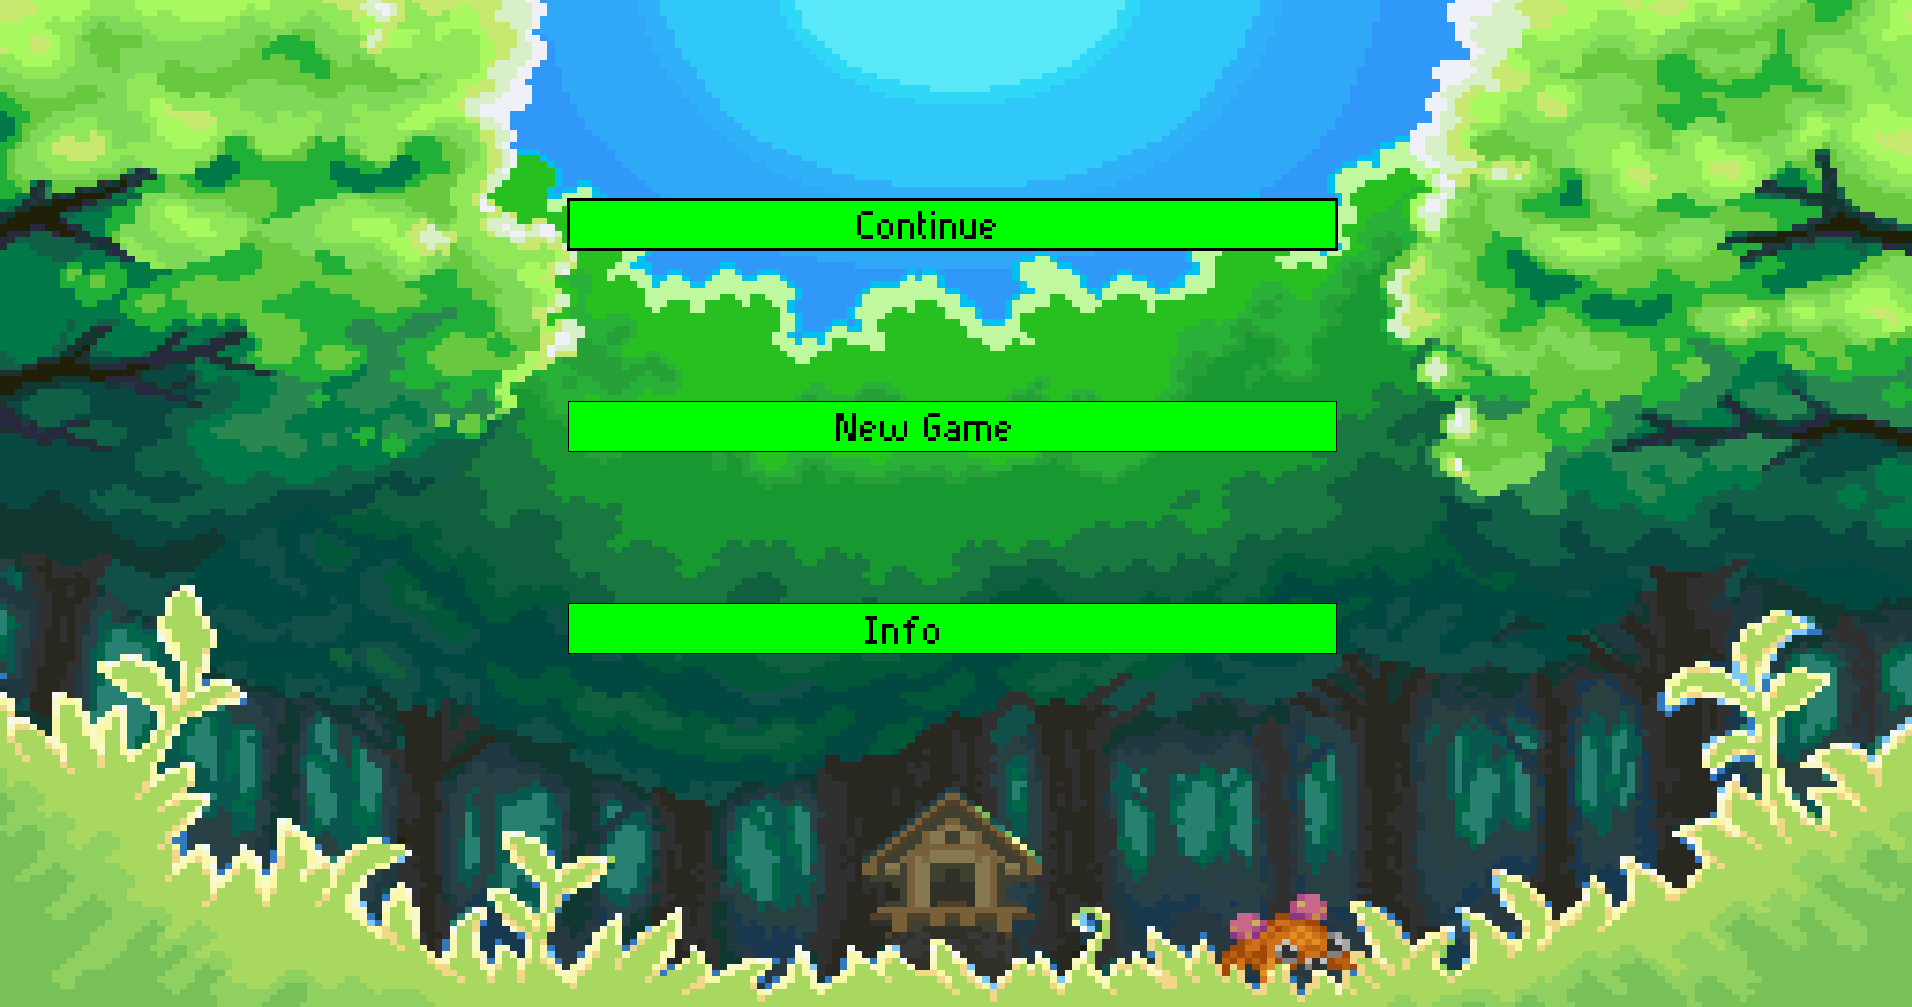
\includegraphics[width=\textwidth]{immagini/scermataHome.png}
  \caption{Schermata principale del gioco al lancio dell'applicazione}
    \label{fig:scermataHome}

\end{figure}

Dopo l’apertura dell’applicativo, si accede alla schermata principale (vedi Figura ~\ref{fig:scermataHome}).\\
Questa schermata presenta tre opzioni principali:

\begin{itemize}
  \item \textbf{Continue}: consente di riprendere una partita precedentemente salvata (sono presenti salvataggi utili alla demo);
  \item \textbf{New Game}: avvia una nuova partita da zero;
  \item \textbf{Info}: mostra informazioni aggiuntive sul gioco.
\end{itemize}

Per iniziare una nuova partita, selezionare l’opzione \texttt{New Game} e premere \textbf{Invio}.\\
Se si desidera esplorare i salvataggi disponibili ad esempio, per sperimentare il funzionamento di elementi specifici come il box, oppure per riprendere una sessione precedente è possibile accedere all’elenco dei salvataggi tramite l’opzione \texttt{Load Game}, disponibile una volta selezionato \texttt{Continue}.


\section{Selezione vecchio salvataggio}

\begin{figure}[H]
  \centering
  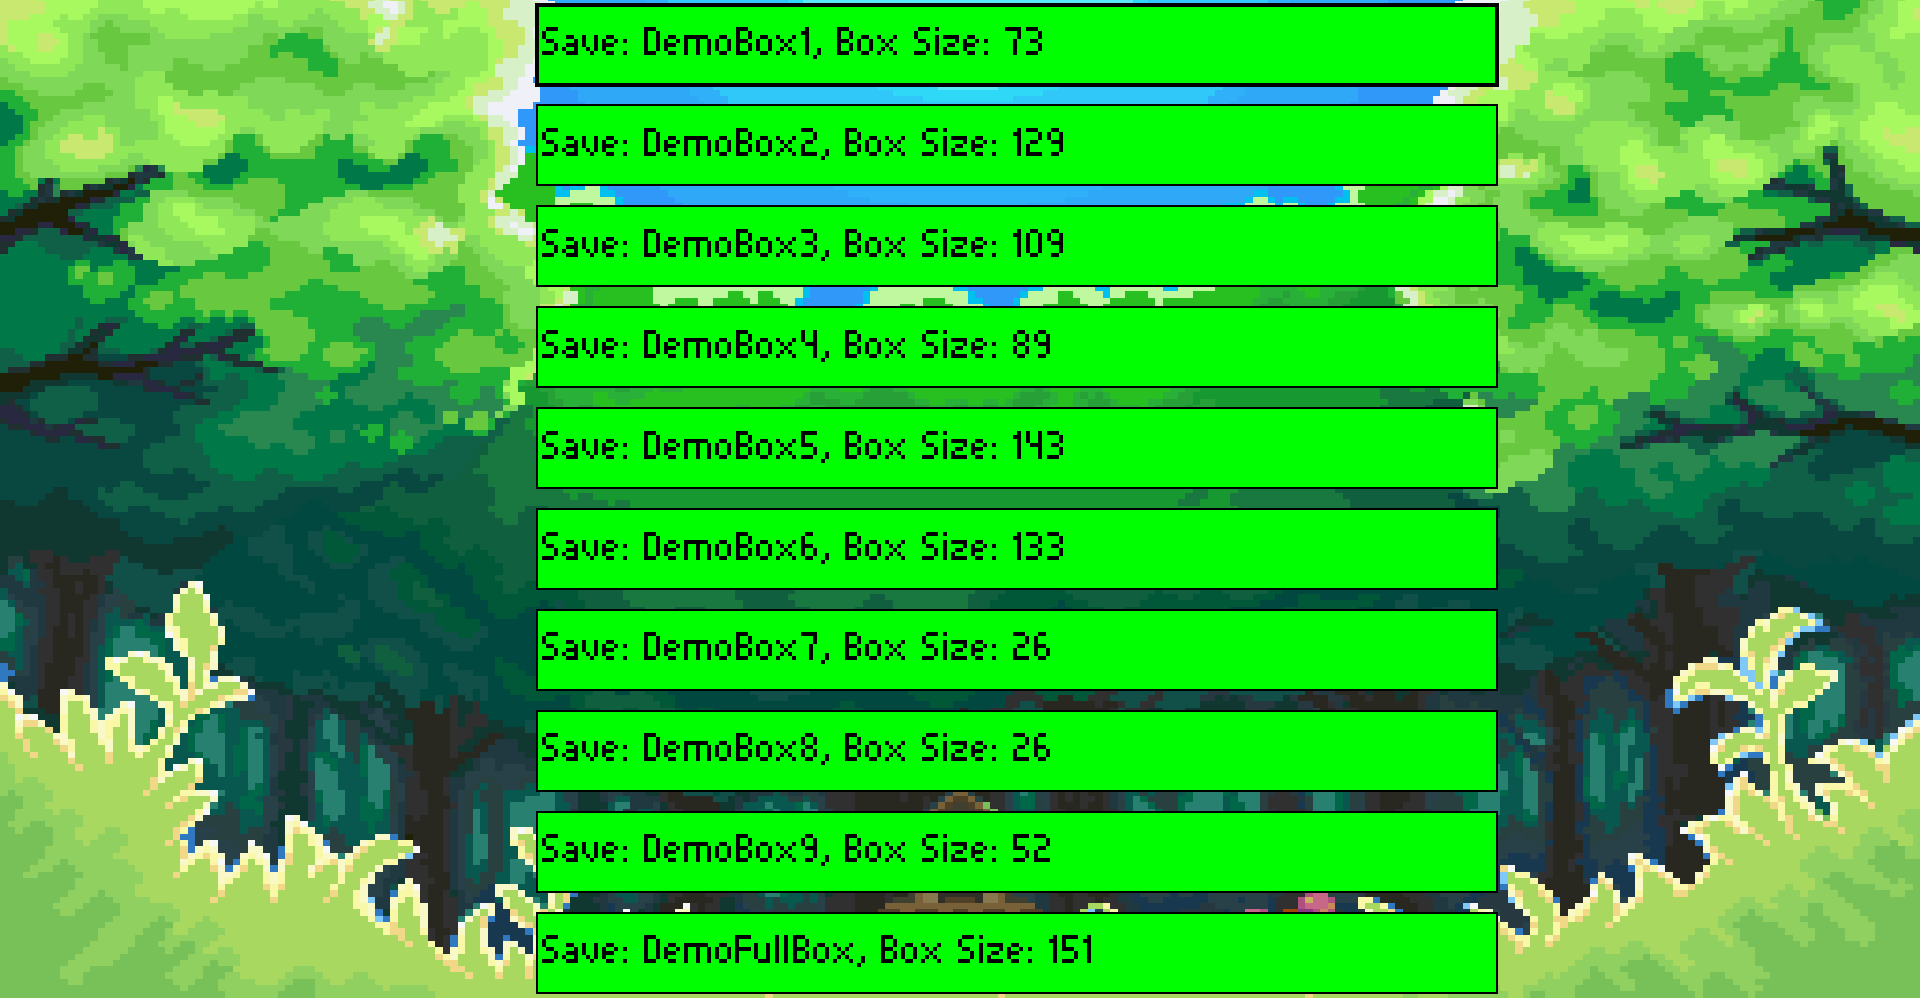
\includegraphics[width=\textwidth]{immagini/schermataLoad.png}
  \caption{Visualizzazione dei salvataggi}
  \label{fig:load_screen}
\end{figure}

Nel menu di selezione del salvataggio sono visibili la dimensione (ovvero il numero di Pokémon sbloccati) e il nome del salvataggio.\\
Sono presenti più schermate di salvataggi, se si hanno più di 9 salvataggi, raggiungendo l’ultimo salvataggio visibile e premendo nuovamente il tasto freccia giù, si accederà a una nuova schermata con altri salvataggi.\\
Per tornare indietro al menu, solo in questa scena, è possibile premere il tasto \textbf{Backspace}.


\section{Scelta del proprio team}

Prima di iniziare una run, viene sempre visualizzata una schermata in cui bisognerà formare il proprio team. (Figura~\ref{fig:pokemon_panorama}).\\
Posizionandosi con il cursore su un Pokémon, vengono mostrate le sue caratteristiche.


\begin{figure}[H]
  \centering
  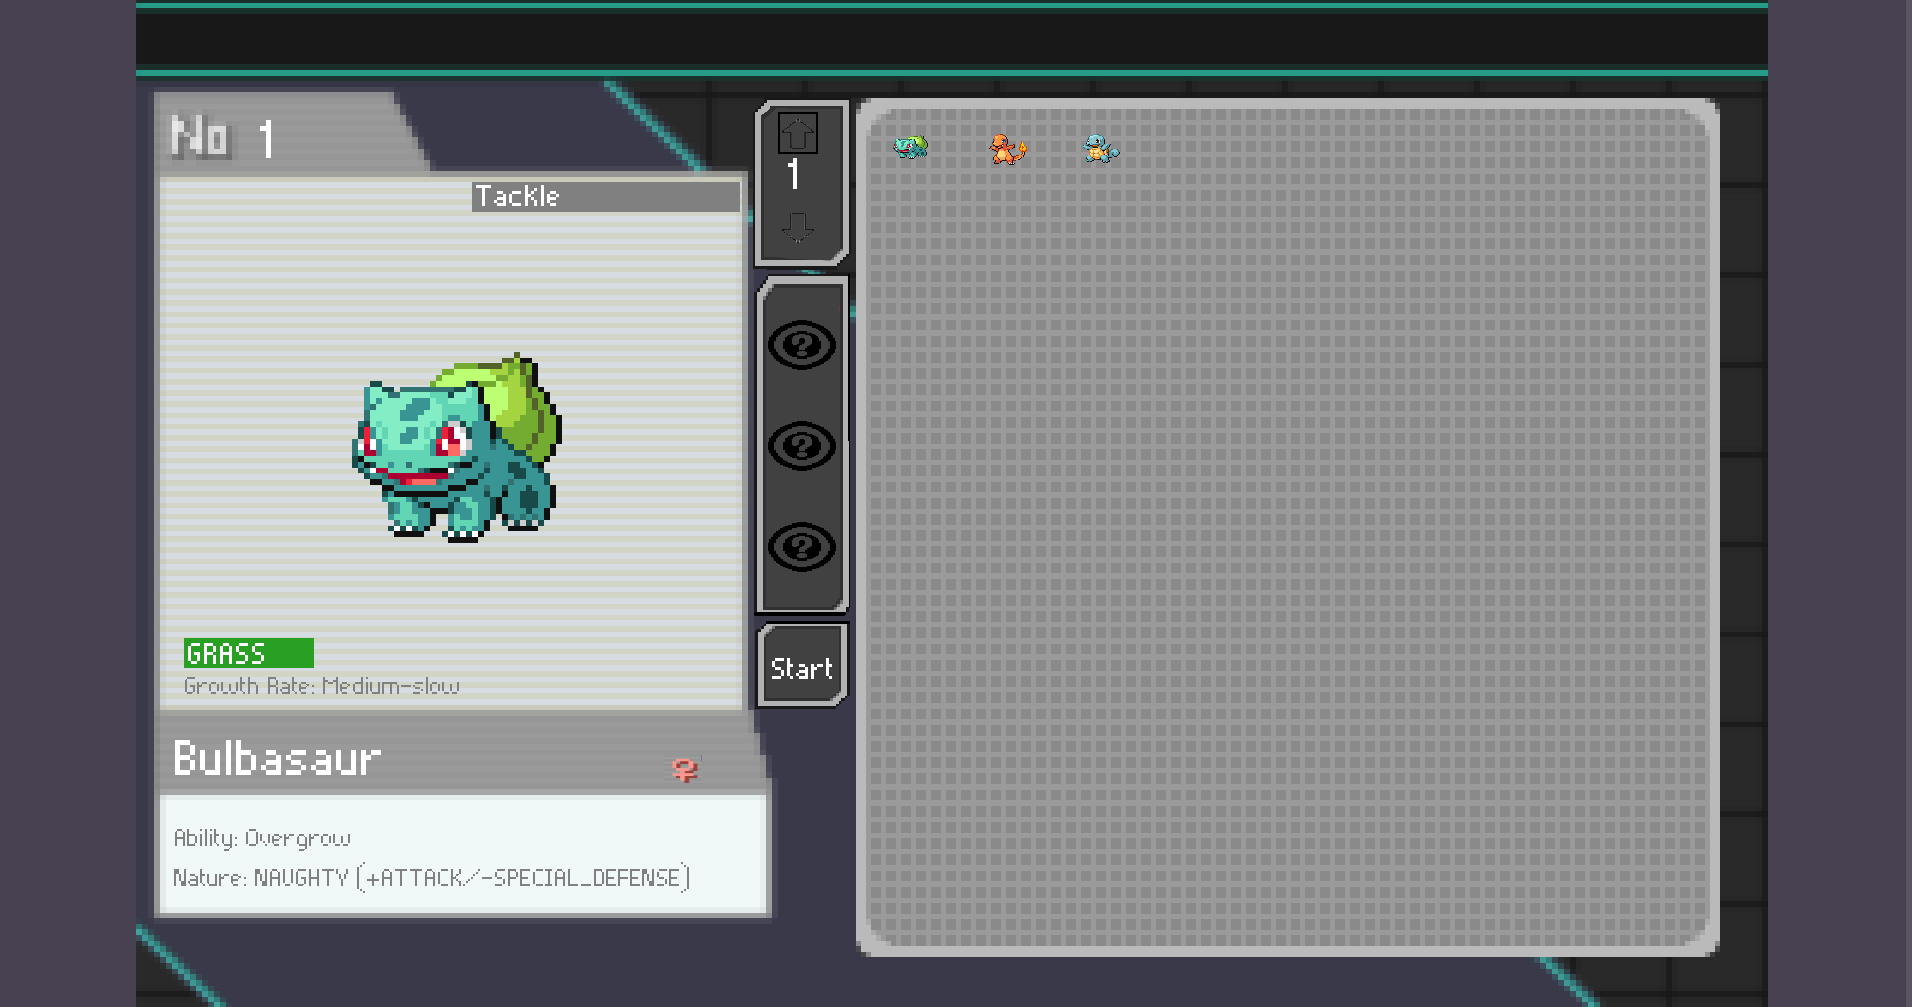
\includegraphics[width=\textwidth]{immagini/schermataBox.png}
  \caption{Immagine rappresentativa del Box contenente i primi tre Pokémon che vengono dati di base iniziando una nuova partita.}
  \label{fig:pokemon_panorama}
\end{figure}

Nel caso in cui si carichi un salvataggio in cui sono stati catturati altri Pokémon durante partite precedenti, anche questi verranno mostrati e potranno essere selezionati.\\
Tuttavia, verranno rigenerati con statistiche differenti e partiranno dal livello 1.\\
Una volta scelto un Pokémon, premere \textbf{Invio} per aggiungerlo alla squadra: occuperà uno dei tre slot disponibili sopra al pulsante \textbf{Start}.\\
È possibile rimuovere un Pokémon selezionato premendo \textbf{Invio} sullo slot che occupa.\\
Se la prima schermata del Box è piena, si può navigare tra le altre pagine utilizzando i bottoni a forma di freccia; il numero visualizzato all’interno di ciascun bottone indica la pagina corrente.\\
Dopo aver selezionato almeno un Pokémon, è possibile premere il pulsante \textbf{Start} per avviare il gioco.


\section{Fase di Combattimento}

Una volta avviato il round, l’utente accede alla fase di combattimento, durante la quale i Pokémon si affrontano.

\begin{figure}[H]
  \centering
  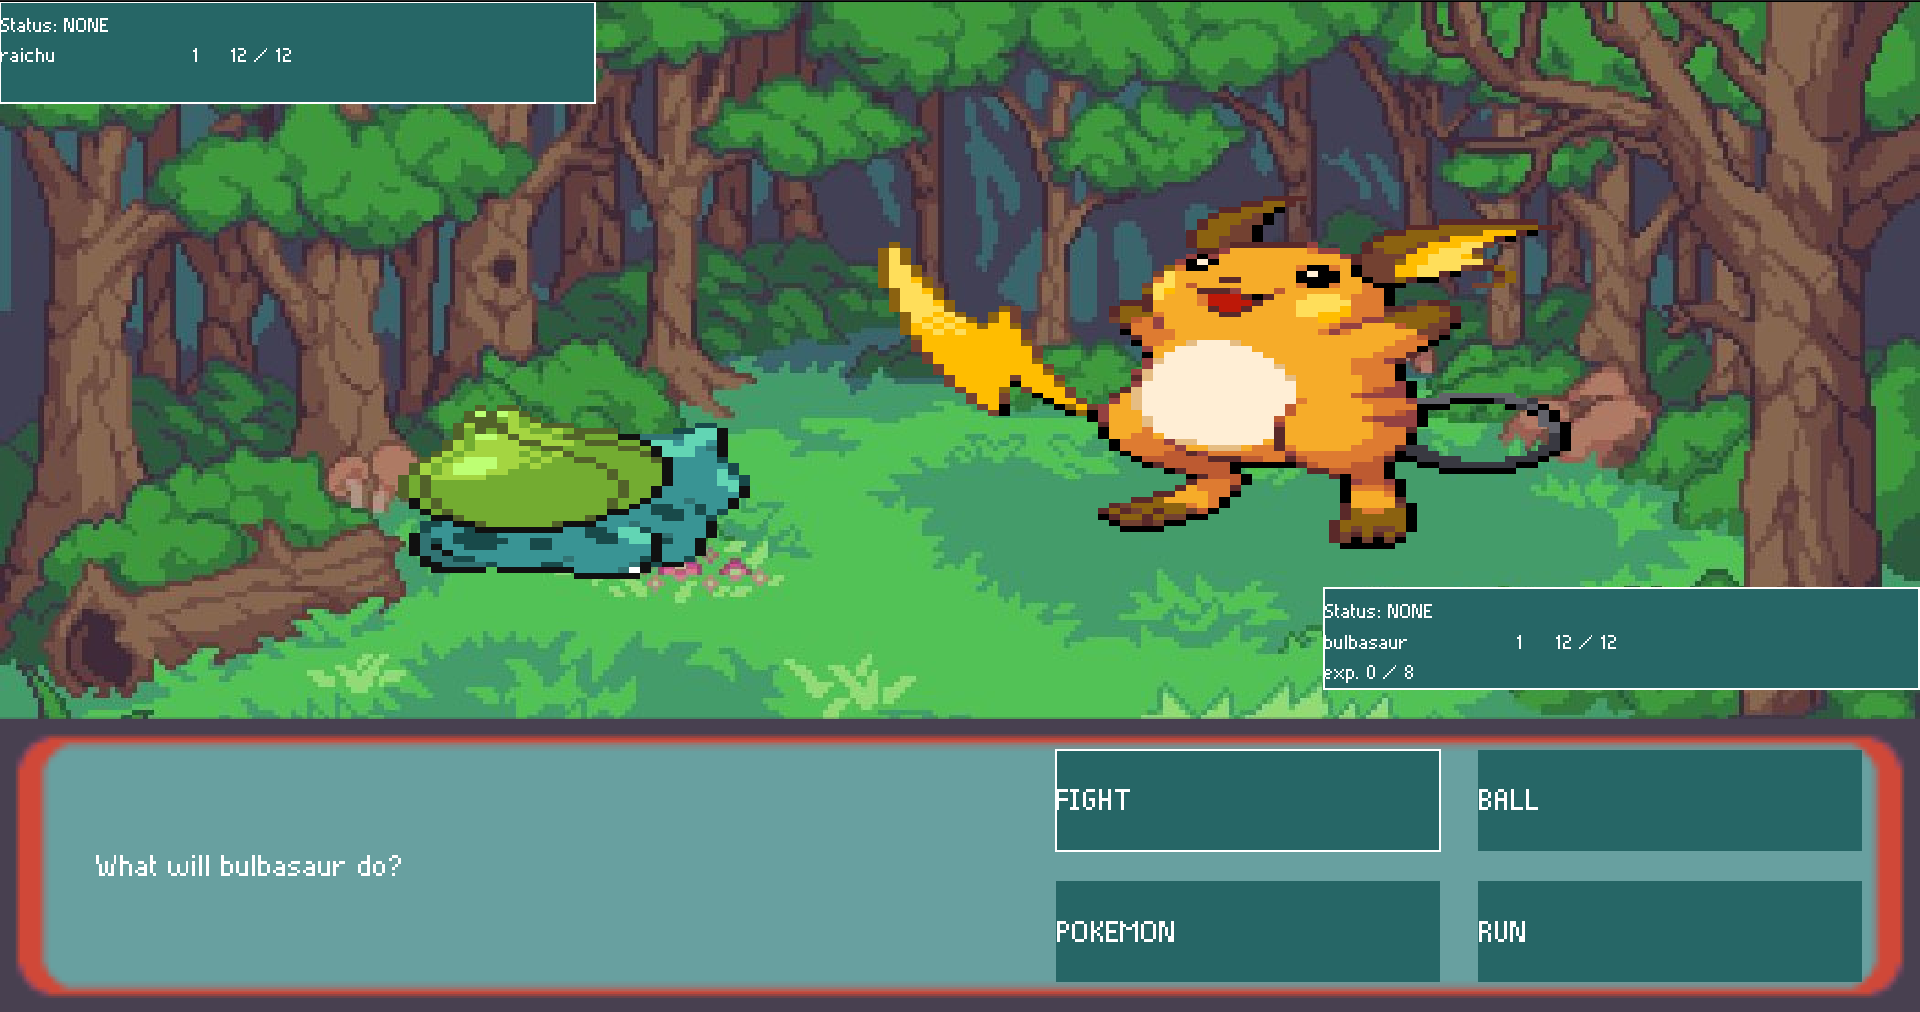
\includegraphics[width=\textwidth]{immagini/schermataFight.png}
  \caption{Visualizzazione della fase di combattimento}
  \label{fig:combat_phase}
\end{figure}

Il riquadro a destra mostra le statistiche del proprio Pokémon. Un valore particolarmente importante da monitorare durante tutta la battaglia è la vita del Pokémon, rappresentata nell’immagine dal valore \texttt{12/12}. Quando la vita raggiunge \texttt{0/12}, il Pokémon non sarà più utilizzabile e verrà automaticamente sostituito con il primo Pokémon disponibile nella squadra.\\
Nel caso in cui non ci siano altri Pokémon disponibili, si tornerà direttamente al \textbf{menu} iniziale senza possibilità di salvare i progressi.\\
È importante considerare anche lo \textit{Status} del Pokémon, anch’esso visibile nel riquadro delle statistiche: questo può influenzare le scelte strategiche durante il combattimento, ad esempio causando danni aggiuntivi o annullando l’efficacia degli attacchi, rendendo alcune azioni inefficaci.\\
Gli Status possono essere applicati tramite abilità passive del Pokémon avversario oppure come effetto delle mosse, e durano per diversi turni.
A destra sono disponibili quattro opzioni, rappresentate da pulsanti rettangolari:
\begin{itemize}
  \item \textbf{FIGHT}: consente di attaccare utilizzando una delle mosse del Pokémon. Inizialmente, ogni Pokémon avrà a disposizione una sola mossa, ma con l’aumentare del livello se ne sbloccheranno di nuove. Ogni mossa ha un numero limitato di utilizzi (PP), che possono essere ricaricati tramite oggetti acquistabili nello Shop.\\
  Se si tenta di attaccare con una mossa esaurita (PP pari a 0), l’attacco non avrà effetto e il Pokémon nemico eseguirà comunque la propria azione.\\
  
  \begin{figure}[H]
    \centering
    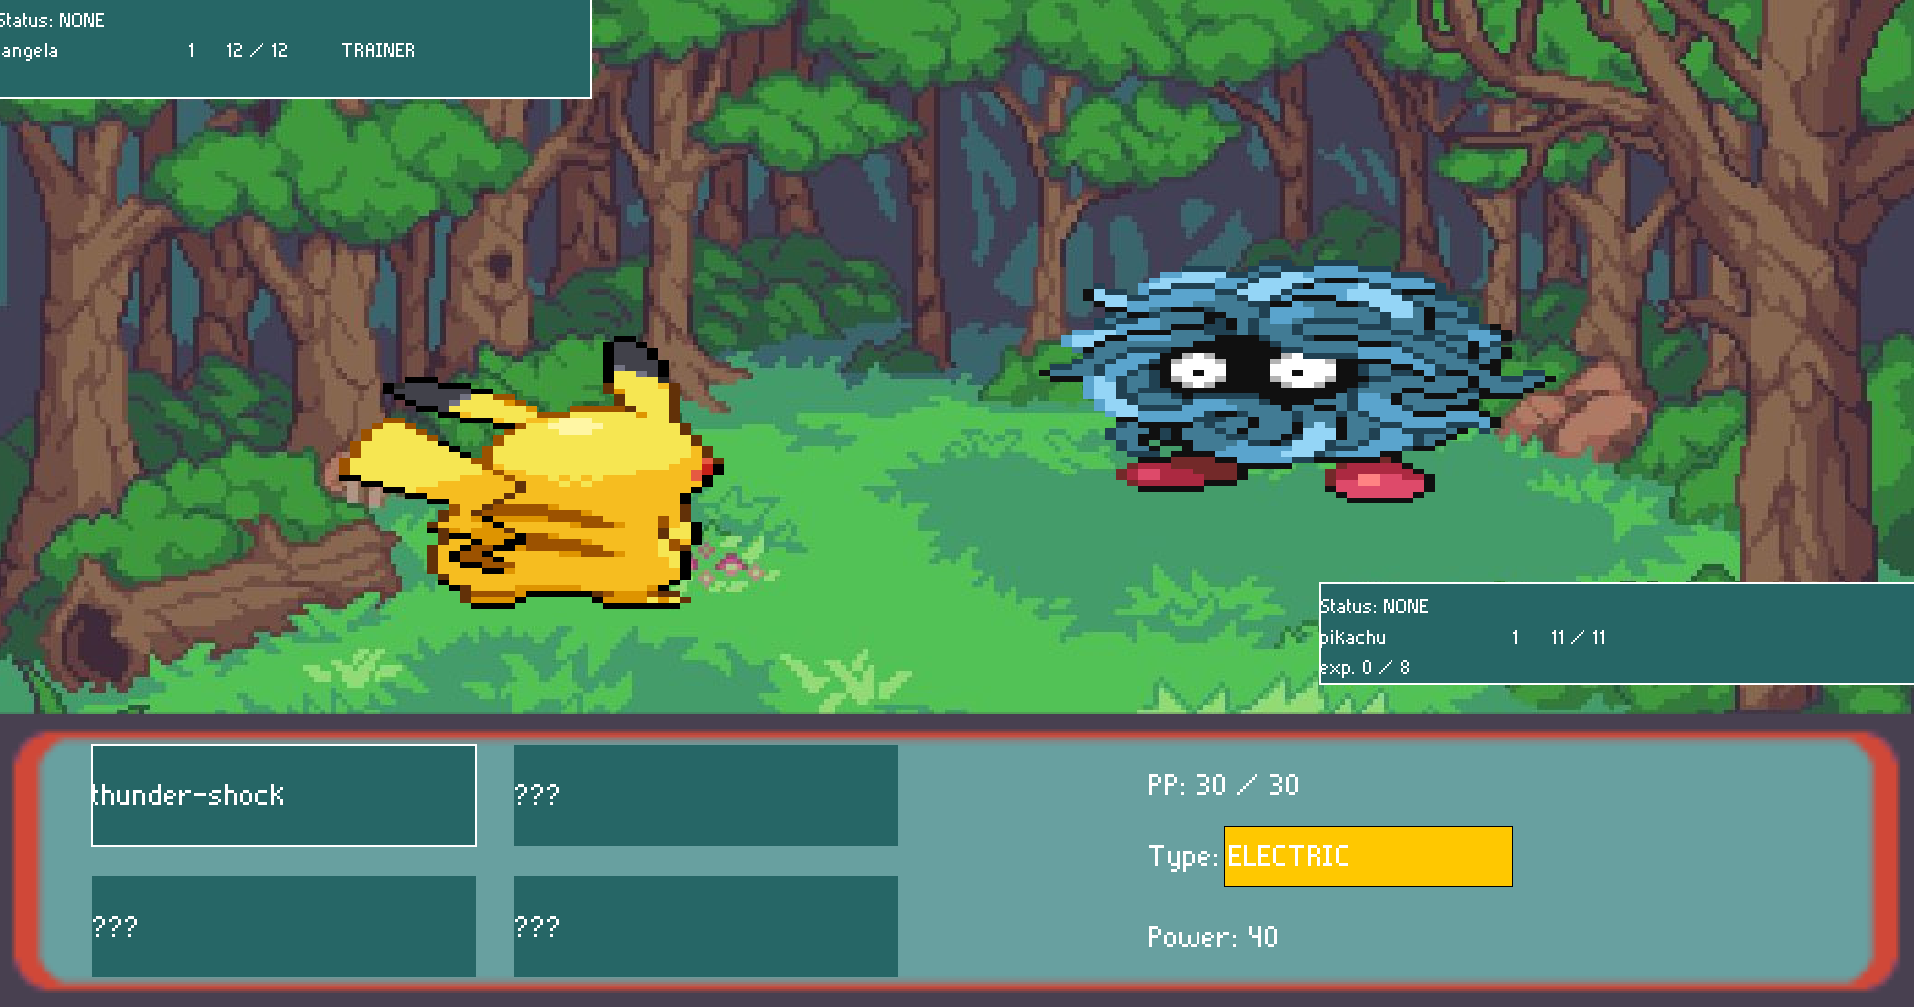
\includegraphics[width=\textwidth]{immagini/moveImg.png}
    \caption{Le mosse non ancora sbloccate vengono visualizzate come "???": è possibile selezionarle, ma non avranno alcun effetto. Il Pokémon nemico, se in grado, attaccherà comunque.}
    \label{fig:move_display}
  \end{figure}

  \item \textbf{BALL}: permette di tentare la cattura del Pokémon avversario.\\
  Tuttavia, se si affronta un allenatore (identificabile dal tag \textbf{TRAINER} visibile nel riquadro delle statistiche in alto a sinistra), la cattura non sarà possibile: in questo caso, le Poké Ball non diminuiranno.\\
  Se la cattura va a buon fine e vi è spazio nella squadra, il Pokémon catturato ne entrerà a far parte. In caso contrario, verrà comunque registrato nel salvataggio, solo se non è già presente nel Box iniziale.\\
  Ogni tentativo di cattura consuma un turno, quindi, se il Pokémon nemico non viene catturato, potrà comunque eseguire la propria azione. Importante notare che catturare un Pokémon aumenta l'esperienza del proprio Pokèmon in campo, il che può portare a un level up.

  \begin{figure}[H]
    \centering
    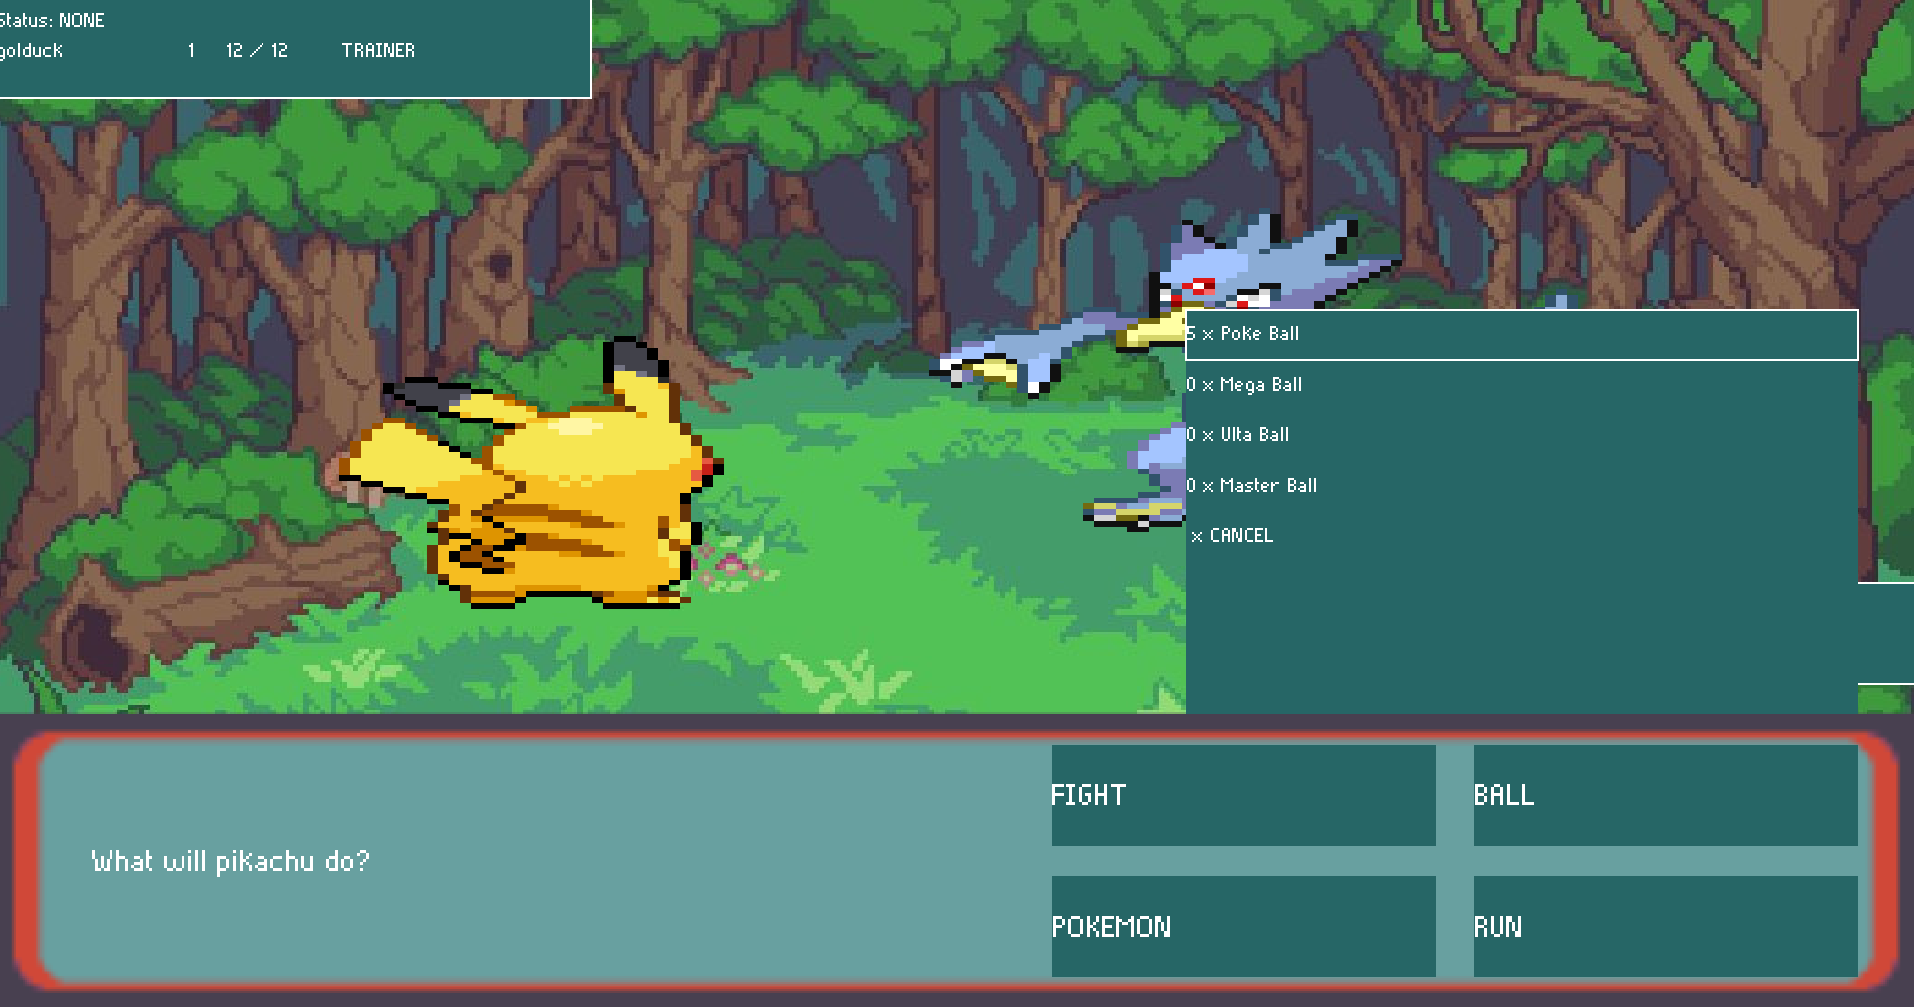
\includegraphics[width=\textwidth]{immagini/ballImg.png}
    \caption{Ogni partita inizia con cinque Poké Ball e una Master Ball. Ogni Poké Ball ha una probabilità di cattura diversa, dalla più bassa alla più alta, con la Master Ball che garantisce la cattura sicura.}
    \label{fig:ball_display}
  \end{figure}

  \item \textbf{POKEMON}: consente di cambiare il Pokémon attivo con un altro del proprio team, a patto che sia ancora in vita. Per effettuare il cambio, selezionare il Pokémon desiderato e premere \textbf{Invio}. Dopo il cambio, il Pokémon nemico eseguirà la propria azione.

  \begin{figure}[H]
    \centering
    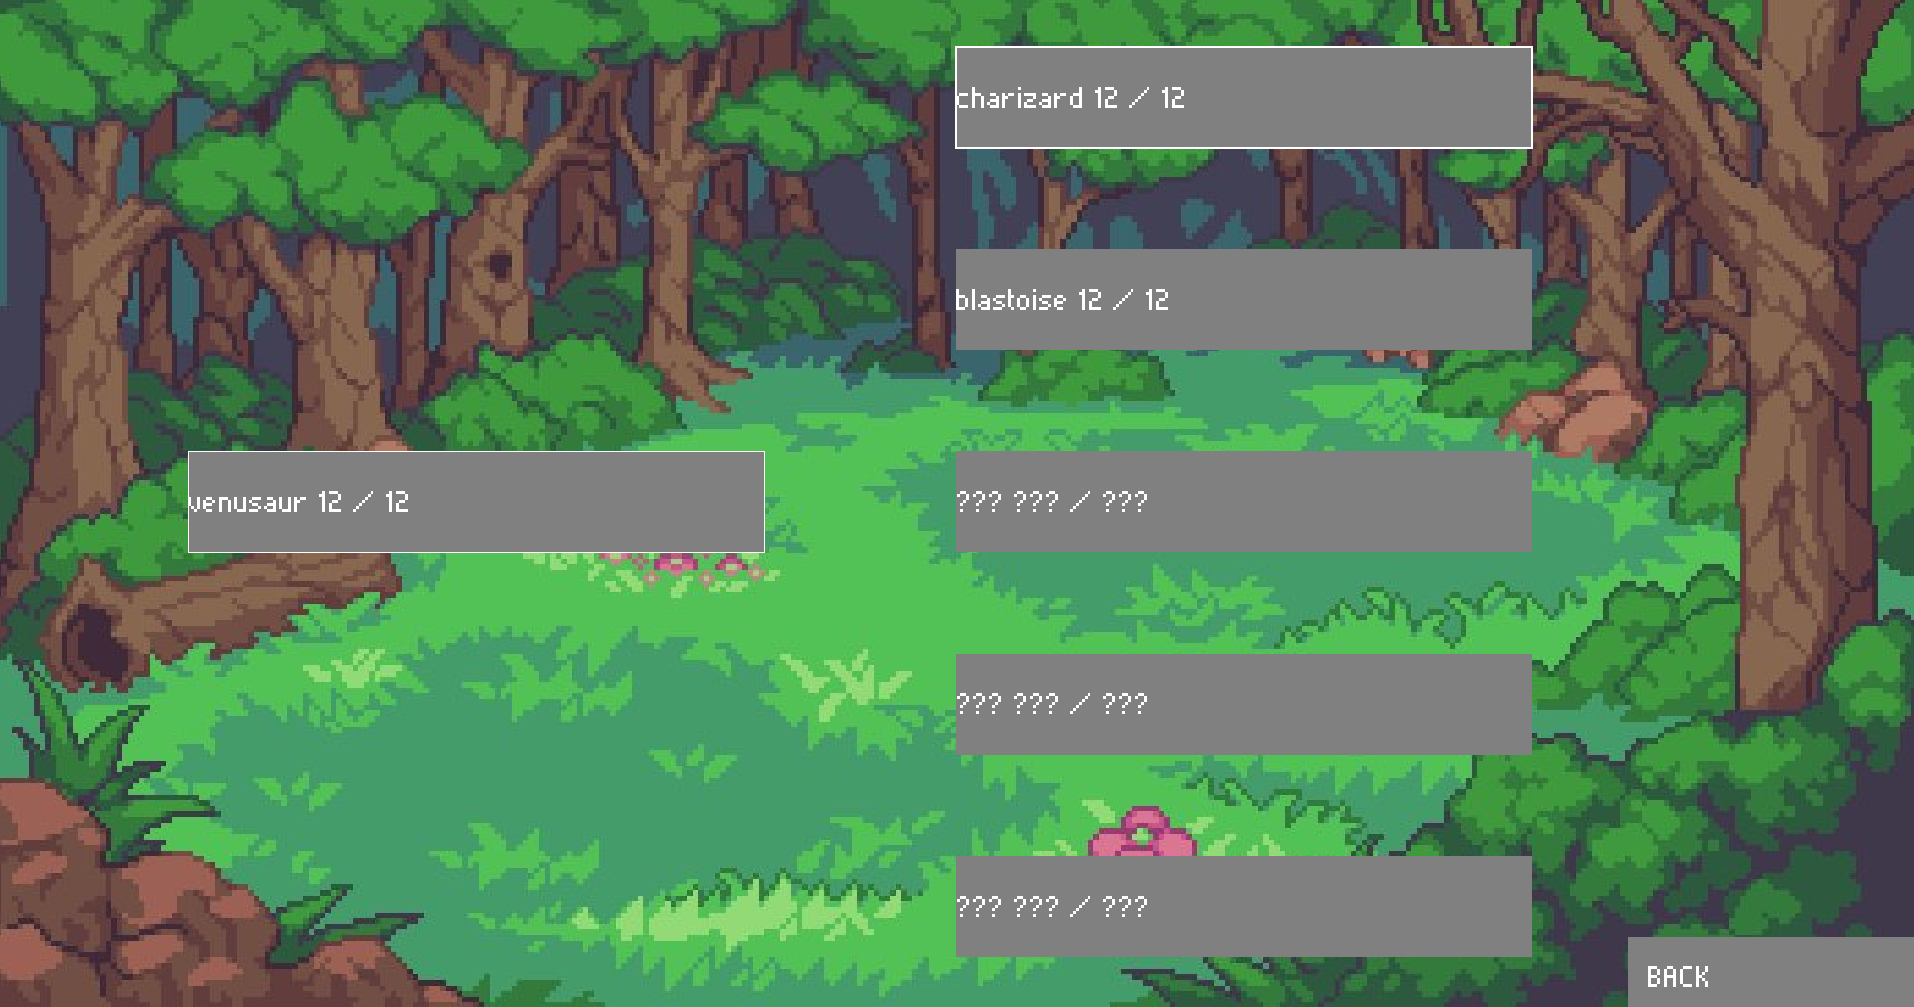
\includegraphics[width=\textwidth]{immagini/changePoke.png}
    \caption{Gli spazi vuoti nella squadra vengono visualizzati come "???". È possibile selezionarli, ma non avranno effetto. Quando nuovi Pokémon vengono catturati, andranno a riempire questi slot.}
    \label{fig:pokemon_change}
  \end{figure}

  \item \textbf{RUN}: consente di saltare il turno.
\end{itemize}
Proseguendo nel gioco, quando un Pokémon raggiunge determinati livelli, imparerà nuove mosse.\\
Le prime tre mosse apprese verranno aggiunte automaticamente al suo set.\\
A partire dalla quarta mossa, invece, sarà richiesto l’intervento dell’utente.\\
In questi casi, comparirà una schermata che permetterà al giocatore di sostituire una delle mosse attualmente conosciute con la nuova mossa disponibile.
Se si desidera mantenere le mosse già apprese, sarà sufficiente premere \textbf{Invio} sulla nuova mossa per rifiutarla e tornare al gioco senza effettuare modifiche.\\
Dopo questa scelta, si verrà riportati alla fase di combattimento, nel caso si stia affrontando un allenatore con altri Pokémon ancora in vita; altrimenti, si accederà direttamente allo \textit{Shop}.

\begin{figure}[H]
  \centering
  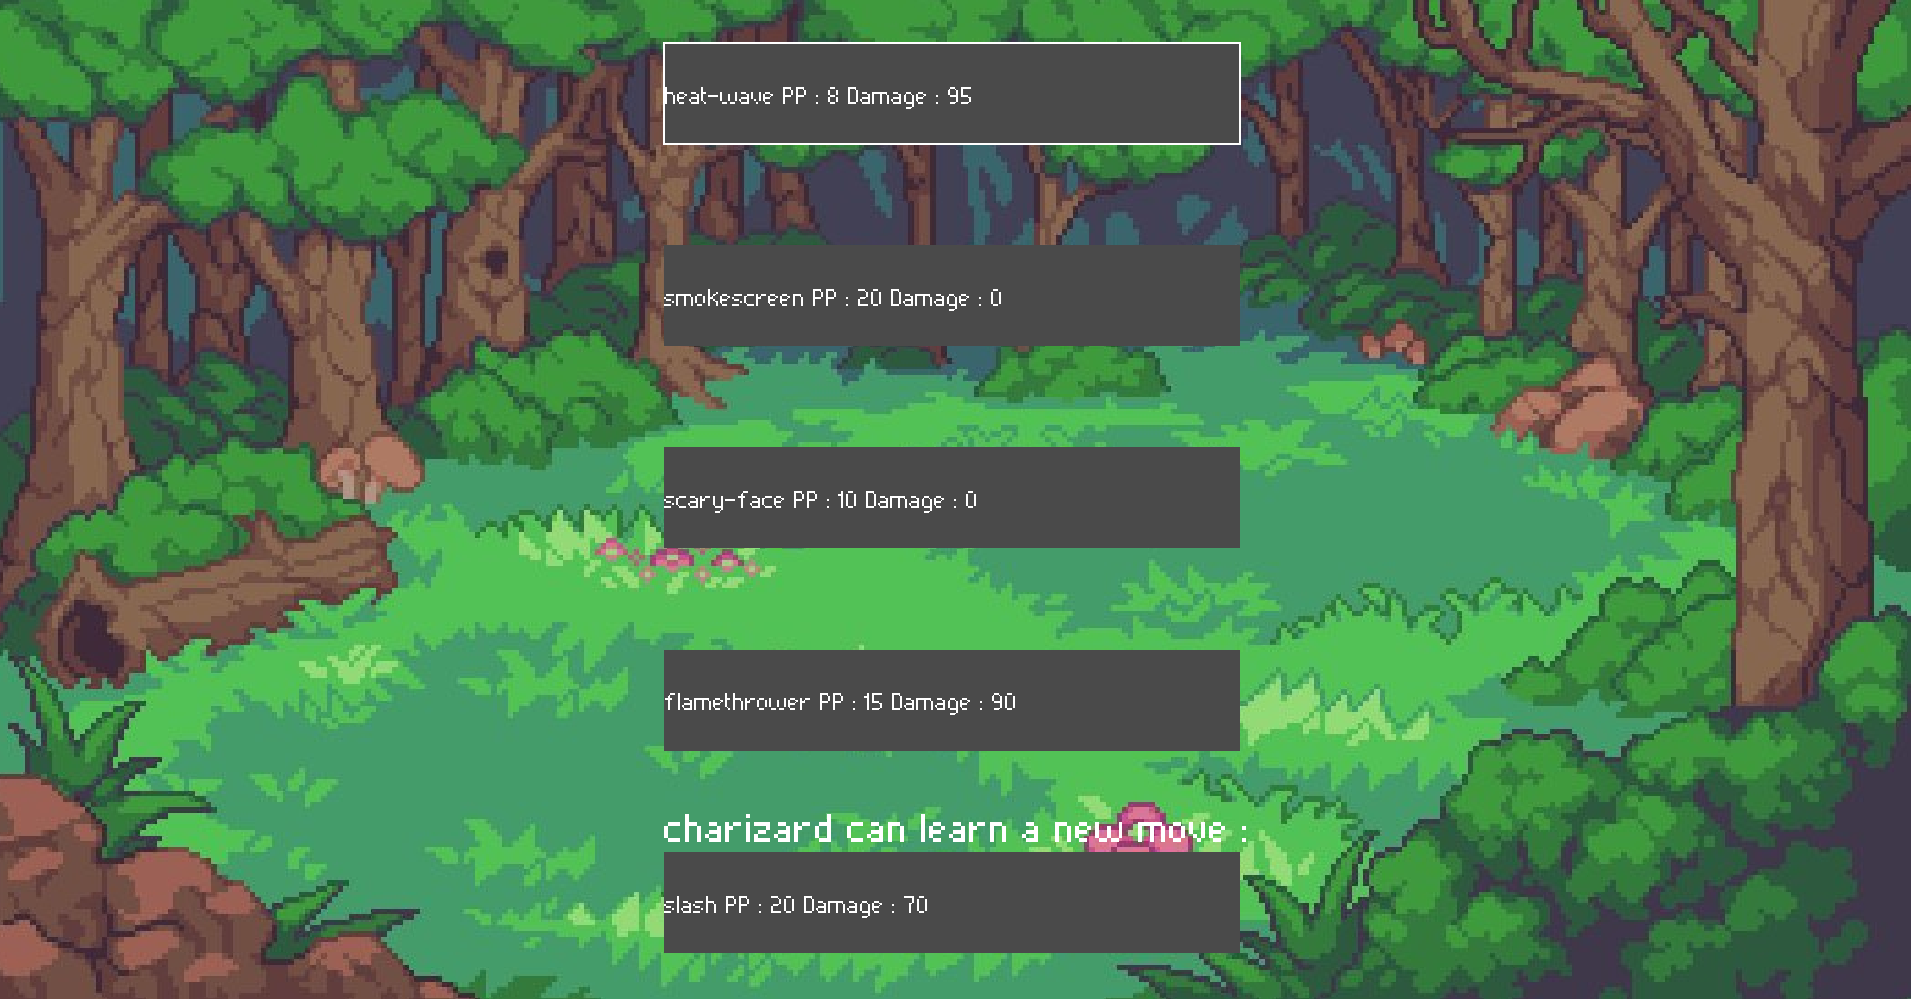
\includegraphics[width=\textwidth]{immagini/NewMoveToLearn.png}
  \caption{Schermata per lo sblocco di nuove mosse}
  \label{fig:save_screen}
\end{figure}
\noindent
È importante ricordare che i nemici con il tag \textbf{TRAINER} dispongono di una squadra di Pokémon: sarà necessario sconfiggerli tutti per poter accedere allo Shop.

\begin{figure}[H]
  \centering
  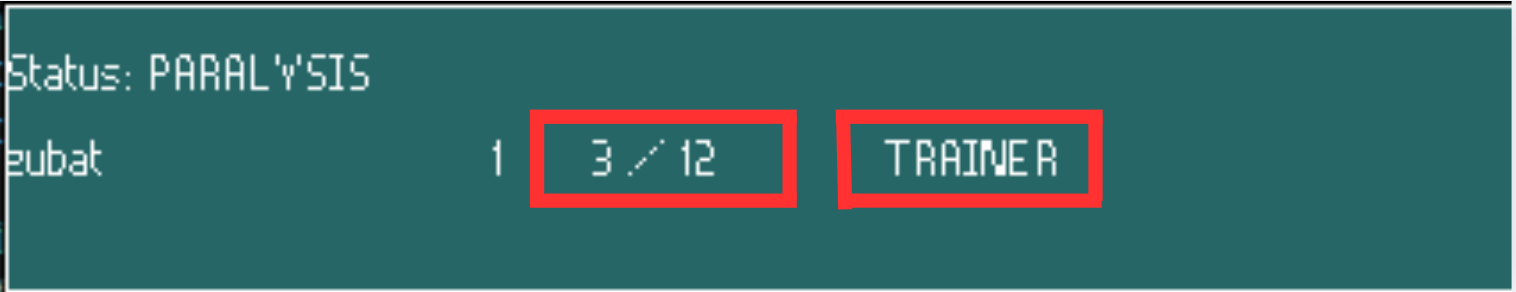
\includegraphics[width=\textwidth]{immagini/Trainer.png}
  \caption{Visualizzazione del tag \textbf{TRAINER} e della vita del Pokémon nemico.}
  \label{fig:trainer_tag}
\end{figure}

\section{Shop}

Dopo aver vinto la fase di combattimento, il giocatore accede allo \textit{Shop}, dove può acquistare oggetti utili per i round successivi.\\
È possibile acquistare un solo oggetto per volta. Alcuni oggetti richiedono di essere applicati direttamente a un Pokémon: in tal caso, verrà aperto un menu con una meccanica simile a quella del pulsante \textbf{POKEMON}.

\begin{figure}[H]
  \centering
  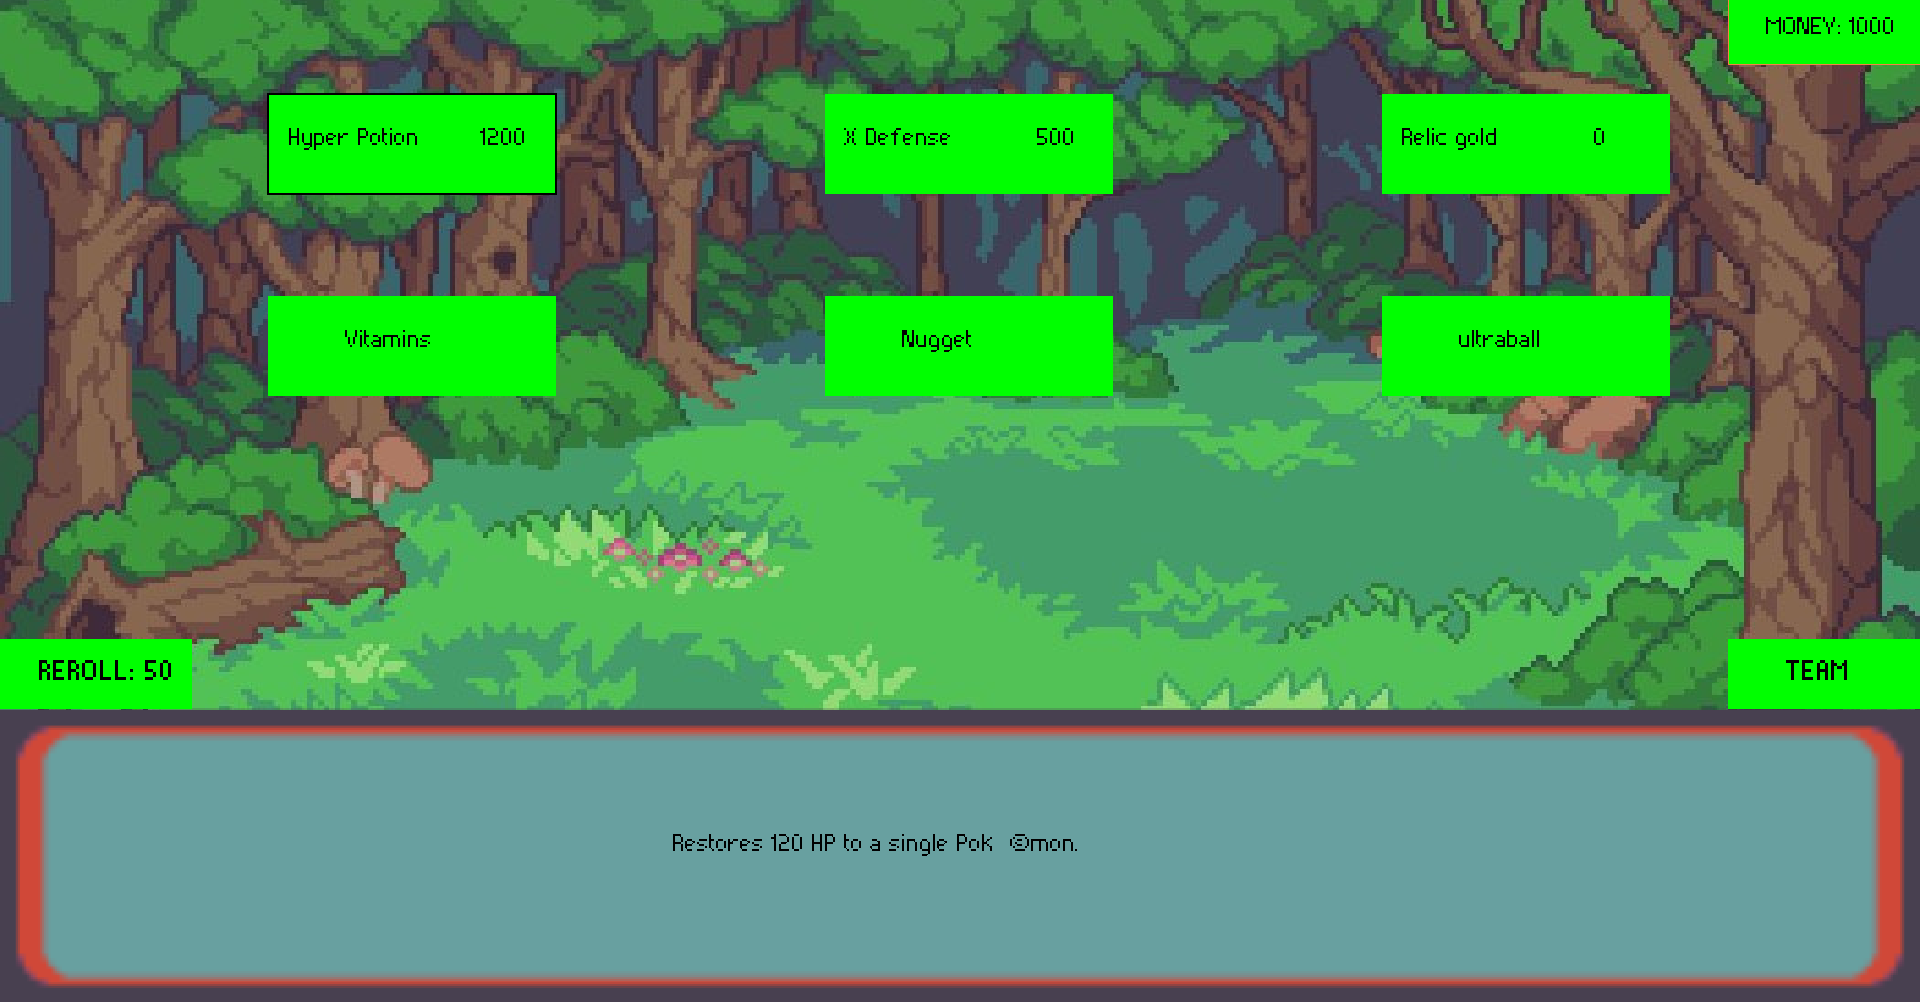
\includegraphics[width=\textwidth]{immagini/schermataShop.png}
  \caption{Visualizzazione della schermata dello shop.}
  \label{fig:shop_screen}
\end{figure}

Nella \textbf{parte superiore destra} è visualizzato il totale di denaro a disposizione del giocatore, mentre al centro sono disposti i vari oggetti acquistabili, ciascuno rappresentato dal nome e dal relativo prezzo.\\
Gli oggetti si dividono in gratuiti e a pagamento (con prezzo visibile); gli oggetti a pagamento sono acquistabili solo se si dispone di abbastanza denaro.\\
Nella \textbf{parte inferiore sinistra} è presente il pulsante \texttt{REROLL}, che permette di aggiornare casualmente gli oggetti in vendita al costo di 50 monete. Anche questo pulsante è utilizzabile solo se si ha sufficiente denaro.\\
Nella \textbf{parte inferiore destra} si trova il pulsante \texttt{TEAM}, che consente di accedere alla schermata della propria squadra per osservare i Pokémon disponibili prima di scegliere l’oggetto più adatto alle proprie esigenze.\\
Infine, nella \textbf{parte inferiore centrale} è presente un riquadro descrittivo che mostra informazioni dettagliate sull’oggetto attualmente selezionato, aiutando il giocatore nella scelta d’acquisto.


\newpage
\section{Salvataggio}
Dopo il decimo combattimento, si aprirà la schermata di salvataggio.

\begin{figure}[H]
  \centering
  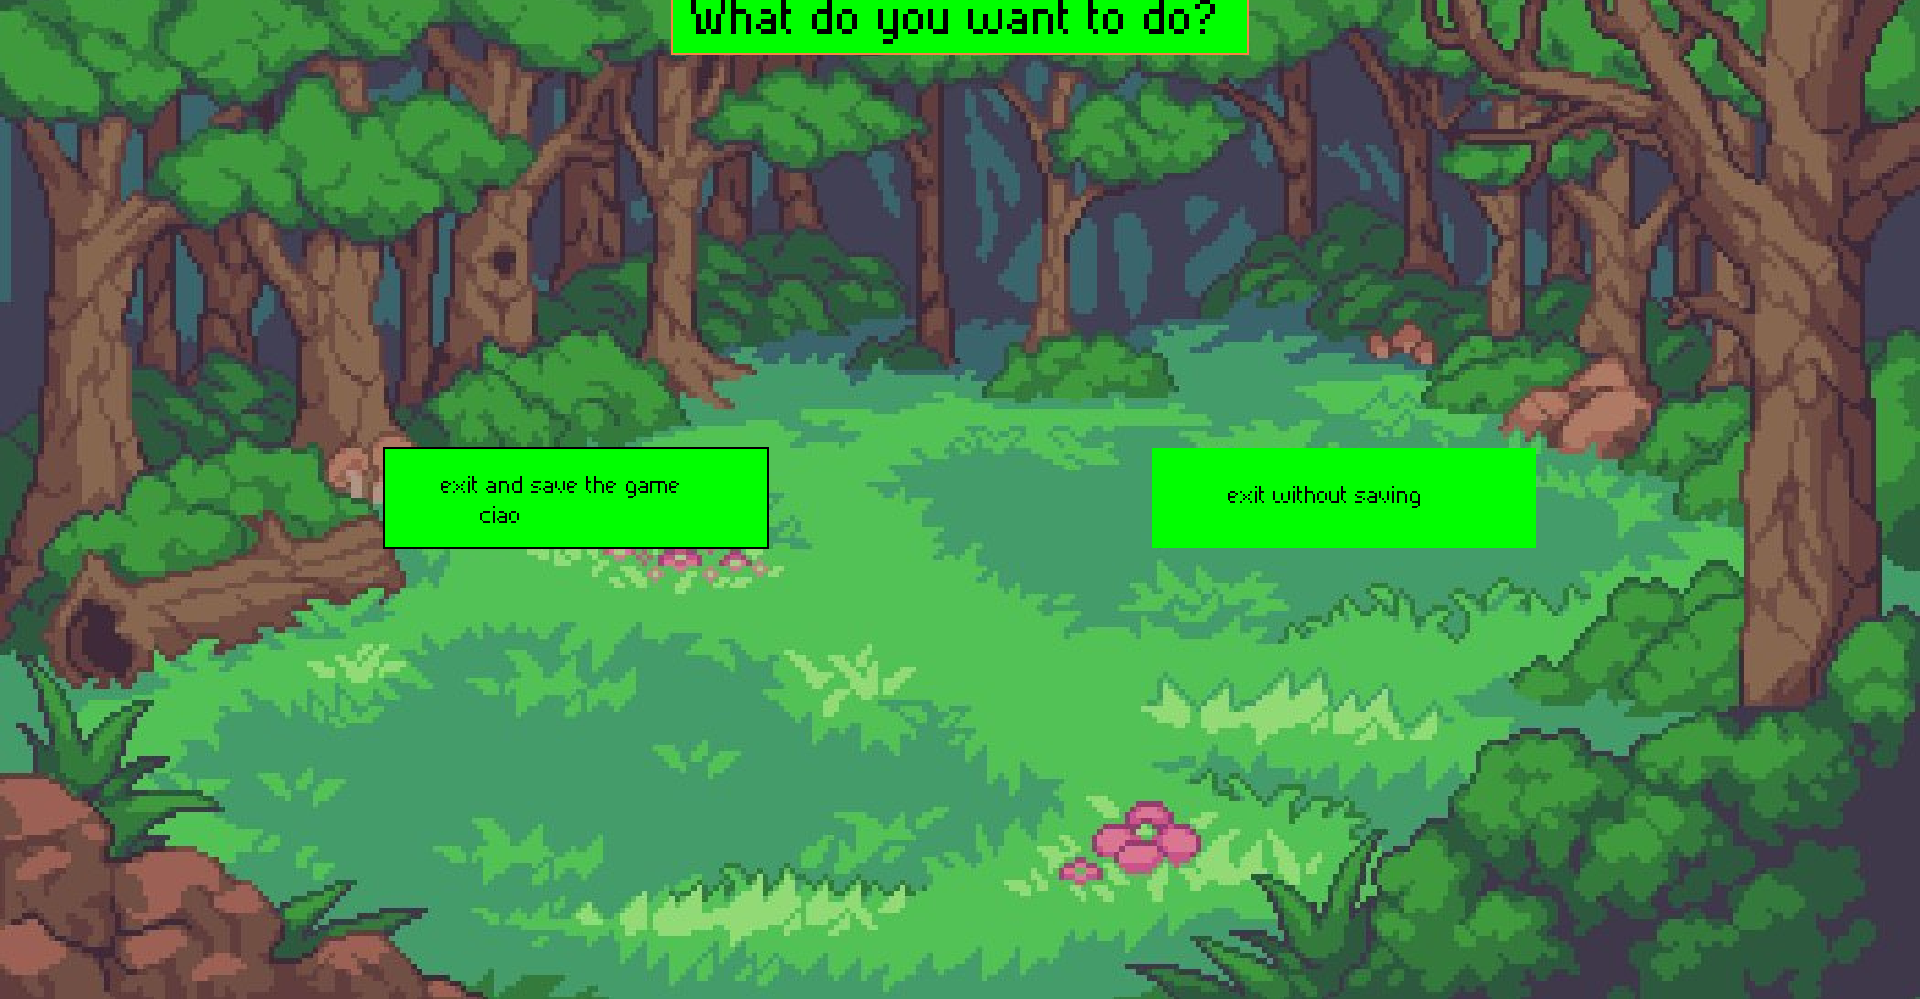
\includegraphics[width=\textwidth]{immagini/schermataSalvataggio.png}
  \caption{Visualizzazione della schermata di salvataggio.}
  \label{fig:save_screen}
\end{figure}



Nel \textbf{pulsante a sinistra} è visualizzato il nome del salvataggio, che va scritto dall'utente tramite tastiera, sarà possibile usare ogni carattere, numero, spazi e sarà possibile cancellare ciò che si ha scritto utilizzando  \textbf{backspace}, con lunghezza in caratteri compresa tra 1 e 12, una volta scritto il nome basterà premere invio sul bottone e verrà creato un nuovo salvataggio, nel caso il nome sia già presente oppure non rispetti i limiti di dimensione non sarà possibile salvare.
Se invece si desidera uscire senza salvare la partita basterà utilizzare il \textbf{pulsante a destra}. Ogni decisione presa ti riporterà al Menù principale del gioco.\\

\subsection*{Versione Demo}

Nella versione Demo sono state apportate alcune modifiche mirate a facilitare e velocizzare il processo di test:

\begin{itemize}
    \item \textbf{Incremento dell’esperienza ottenuta}: i punti esperienza (EXP) guadagnati durante le battaglie sono stati aumentati, così da permettere un avanzamento di livello più rapido.
    
    \item \textbf{Sblocco anticipato delle mosse per gli starter}: i tre Pokémon iniziali – \textit{Bulbasaur}, \textit{Charmander} e \textit{Squirtle} – ora apprendono tutte le loro prime mosse nei \textbf{primi 6 livelli}. Questo intervento ha lo scopo di consentire il test completo della scena di \textit{selezione delle mosse}, permettendo al giocatore di decidere quali mantenere già nelle fasi iniziali del gioco.
\end{itemize}

\end{document}
